\chapter{偏微分方程}
\label{chap:partial-differential-equations}

把一根金属细棒的中段加热，再让它在空气中冷却。上一章的状态是有限个数，比如一个房间的平均温度；可是这根棒上每一点都有自己的温度，热量还在相邻的点之间流动。要预测“一分钟后棒中点有多热”，只知道中点现在的温度不够，还得知道它两侧的温度怎样弯曲、棒的两端是固定在冰水里还是包着隔热层。未知量由一个向量变成了定义在空间区域上的函数，这样的函数称为场，约束场的方程同时含有对空间和对时间的偏导数。

本章围绕四个问题展开。第一，需要给出哪些数据，一个场才算被方程确定：源项、初始场与边界条件各起什么作用？第二，当场带有尖点、源项只是可积函数甚至集中在一点时，“满足方程”应当怎样解释？第三，扩散、搬运和振动这三种演化机制，各自让场发生了什么变化，哪些量守恒、哪些量衰减、信号传得多快？第四，计算机只能处理有限个未知量，网格上的近似解在什么条件下、以什么速度逼近连续的解？

第~\ref{sec:pde-fields-boundary-data}节先把有限维状态推广为空间场，用同一个初始鼓包比较扩散、输运和波动三种机制，并说明边界数据和“解”的含义必须与方程一同给出。第~\ref{sec:pde-poisson}节研究不含时间的Poisson方程：用测试函数把方程改写成弱形式，借Lax--Milgram定理证明弱解存在唯一，用能量估计说明数据怎样控制解；Neumann与Robin边界将显示，改变边界会改变解空间、相容条件和唯一性。这一节建立的弱形式和能量方法是后面三类演化方程的共同工具。

第~\ref{sec:pde-heat}节把热方程看作函数空间中的连续时间演化：正弦模式按指数衰减、高频衰减更快，能量估计给出唯一性，解算子组成半群，最大值原理和Poincaré不等式刻画正性与长期极限。第~\ref{sec:pde-transport}节沿特征线把输运方程化为上一章的常微分方程，并比较“搬运数值”与“搬运质量”，再用Burgers方程说明特征线交叉时经典解为何失效。第~\ref{sec:pde-wave}节研究需要位移和速度两类初值的波动方程，它以有限速度传播、保持能量，与热方程的瞬时扩散和能量耗散形成对照。第~\ref{sec:pde-discretization}节固定这些方程，研究有限差分与有限元怎样把场变成有限个未知量，再借上一章的时间推进方法求解；空间误差、时间误差与代数求解误差将分开估计。

全章以实值场和线性方程为主线，非线性只在守恒律处作为延伸。所用的偏导数、Laplace算子与散度定理来自多元微积分；弱导数、Sobolev空间、边界迹和Poincaré不等式来自函数空间部分，在第~\ref{sec:pde-boundary-solution-meaning}小节集中回顾；有限维的线性常微分方程、Euler方法与刚性来自第~\ref{chap:ordinary-differential-equations}章。

% 第3章第1节：场、方程与边界数据（从状态向量到空间场；初值、边界条件与解的含义）。

\section{场、方程与边界数据}
\label{sec:pde-fields-boundary-data}

本节先说明未知量怎样从有限个坐标变成空间上的函数，再区分只受空间约束的静态场与随时间变化的演化场。随后讨论边界上可以规定哪些数据、初值与边界在交接处怎样协调，以及“解”可以有几种含义。后面四节分别研究的Poisson、热、输运与波动方程，都要先在这里确定数据和解的意义。

\subsection{从状态向量到空间场}
\label{sec:pde-state-to-field}

\paragraph{一根细棒上的温度}
设一根长为$1$的细棒占据区间$[0,1]$，两端浸在冰水中。棒很细，同一横截面上的温度可以看成相同，于是在时刻$t$，位置$x$处只有一个温度$u(x,t)$。固定时刻$t$，整条曲线$x\mapsto u(x,t)$就是棒在这一时刻的状态。它不是一个数，也不是有限个数，而是区间上的一个函数，我们称这样随位置变化的量为\term{场}（field）。

图~\ref{fig:pde-rod-snapshots}画出了一个初始有两个热点的温度场在几个时刻的样子。蓝色曲线是初始温度，随着时间推移，两个尖峰变矮变宽，最后连成一个平缓的拱形，两端始终保持零度。在$t=0.004$这条曲线上，我们还在$11$个等距网格点处取了样：这$11$个温度组成的向量正是上一章意义下的有限维状态。它只是场的一个近似表示，网格点之间的温度、尖峰的确切形状都被丢掉了；第~\ref{sec:pde-discretization}节再研究这种近似何时可靠。

\begin{figure}[!htb]
  \centering
  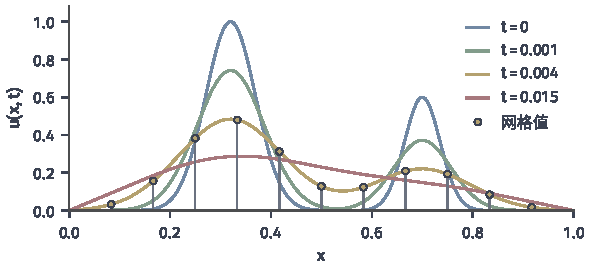
\includegraphics[width=100mm]{figures/03-optimization-evolution-and-signals/02-processes-and-trajectory-evolution/matplotlib/pde-rod-snapshots/figure.pdf}
  \caption{细棒温度场的几个时刻。方程为$u_t=u_{xx}$，两端温度保持为零，初始温度在$x=0.32$与$x=0.7$处各有一个热点。四条曲线是同一个场在不同时刻的整体形状；圆点是$t=0.004$时在$x_j=j/12$（$j=1,\ldots,11$）处取的样，组成一个$11$维向量。曲线由$300$项正弦级数计算。}
  \label{fig:pde-rod-snapshots}
\end{figure}

\paragraph{偏导数读出两种变化}
场$u(x,t)$有两个自变量，变化也有两个方向。固定时刻、沿棒移动，$\partial_xu=u_x$是温度曲线在$x$处的斜率：斜率为正说明右边更热，热量会从右向左流。固定位置、让时间前进，$\partial_tu=u_t$是这一点温度上升或下降的速率。上一章的状态方程规定$\dot{\bm x}$怎样由$\bm x$决定；对场而言，我们要规定$u_t$怎样由$u$在空间上的形状决定，而形状要用$u_x$、$u_{xx}$等空间偏导数来描述。

二阶偏导数有一个直接的读法。设$u$对$x$三次连续可微，由Taylor展开，
\begin{equation}
  \frac{u(x+h,t)+u(x-h,t)}{2}-u(x,t)=\frac{h^2}{2}u_{xx}(x,t)+o(h^2),\qquad h\to0 .
  \label{eq:pde-neighbor-average}
\end{equation}
左边是两侧邻点的平均值减去当前值。所以$u_{xx}>0$表示这一点比邻居的平均值低，曲线在这里向上弯；$u_{xx}<0$表示这一点比邻居高，处在一个凸起上。在$d$维中，Laplace算子$\Delta u=\sum_{i=1}^d\partial_{x_i}^2u$在同样的意义下比较一点的值与周围小球面上的平均值。

\paragraph{静态场与演化场}
并非所有场都随时间变化。一块薄板在固定热源下达到的稳态温度、一张绷紧的膜在固定载荷下的位移、电荷分布产生的静电势，都只依赖位置。这类\term{静态场}（stationary field）只受空间方程约束，例如稳态温度满足$-\Delta u=f$，其中$f$是热源密度；它没有初始时刻，也不需要初值。随时间变化的\term{演化场}（evolving field）则还需要一个起点：热方程要给出初始温度$u(\cdot,0)$，波动方程还要给出初始速度。初值本身是一个函数，这是“状态是函数”的直接后果。

上面这些方程有一个共同的形式：在每一点处，未知函数与它的有限个偏导数满足一个关系。

\begin{definition}[偏微分方程]
\label{def:pde-pde}
设$U\subseteq\mathbb R^n$为开集，$u:U\to\mathbb R$为未知函数。若在每一点$\bm z\in U$处，$u$与它不超过$m$阶的偏导数满足关系
\[
  F\bigl(\bm z,u(\bm z),\nabla u(\bm z),\nabla^2u(\bm z),\ldots,\nabla^mu(\bm z)\bigr)=0,
\]
且$F$确实依赖某个$m$阶偏导数，则称它是$m$阶\term{偏微分方程}（partial differential equation, PDE）。若$F$关于$u$及其各阶偏导数是仿射的，即方程可以写成$Lu=f$，其中$L$是系数只依赖$\bm z$的线性微分算子、$f$是给定函数，则称方程是线性的。
\end{definition}

对演化场，$\bm z=(\bm x,t)$同时包含空间和时间坐标，$n=d+1$。“线性”保证两个解的差满足$f=0$的方程，这一点在后面证明唯一性时反复使用。Burgers方程$u_t+uu_x=0$含有乘积$uu_x$，不是线性的；第~\ref{sec:pde-conservation}小节会看到这一差别带来的后果。

\paragraph{三种变化机制}
同一个初始形状可以按完全不同的方式演化。想象实轴上一个高为$1$的Gauss鼓包，下面三个方程各自让它怎样变化？

第一种是\term{扩散}（diffusion）：$u_t=\kappa u_{xx}$，$\kappa>0$。由式~\eqref{eq:pde-neighbor-average}，变化率正比于“邻居平均值减当前值”：鼓包顶部高于邻居，温度下降；两侧山脚低于邻居，温度上升。结果是峰变矮、形状变宽，总面积保持不变。第二种是\term{输运}（transport）：$u_t+bu_x=0$，$b$为常数。直接验证可知$u(x,t)=u_0(x-bt)$满足方程：形状不变，整体以速度$b$平移，就像河水把一团染料原样带向下游。第三种是\term{波动}（wave）：$u_{tt}=c^2u_{xx}$。这里曲率决定的是加速度而不是速度，顶部被向下拉、获得向下的速度后会越过平衡位置；在初速度为零时，鼓包分裂成两个高度减半的小鼓包，分别以速度$c$向左右跑开。

图~\ref{fig:pde-three-mechanisms}把三种机制并排画出。扩散让信息“抹平”，输运让信息“搬家”，波动让信息“分路传播”。这三幅画面贯穿本章：第~\ref{sec:pde-heat}节证明扩散抹去高频起伏、耗散能量；第~\ref{sec:pde-transport}节沿着平移的轨迹求解输运方程；第~\ref{sec:pde-wave}节说明波动以有限速度传播并保持能量。

\begin{figure*}[!htb]
  \centering
  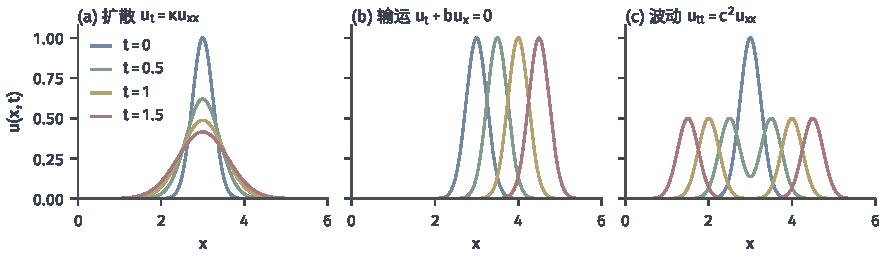
\includegraphics[width=150mm]{figures/03-optimization-evolution-and-signals/02-processes-and-trajectory-evolution/matplotlib/pde-three-mechanisms/figure.pdf}
  \caption{同一初始鼓包$u_0(x)=\exp(-(x-3)^2/(2\cdot0.25^2))$在三种方程下的演化，四种颜色依次为$t=0,0.5,1,1.5$。(a)~扩散，$\kappa=0.1$：解仍是Gauss形，方差由$0.25^2$增大为$0.25^2+2\kappa t$，峰值相应降低。(b)~输运，$b=1$：$u_0(x-t)$原样右移。(c)~波动，$c=1$，初速度为零：$\tfrac12[u_0(x-t)+u_0(x+t)]$，鼓包分为两半向两侧传播。}
  \label{fig:pde-three-mechanisms}
\end{figure*}

\paragraph{二阶方程的分类及其适用范围}
对两个自变量、常系数的二阶线性方程
\[
  a\,u_{yy}+2b\,u_{yz}+c\,u_{zz}+(\text{低阶项})=f,\qquad (a,b,c)\neq(0,0,0),
\]
常按判别式$b^2-ac$的符号分类：小于零称为\term{椭圆型}（elliptic），等于零称为\term{抛物型}（parabolic），大于零称为\term{双曲型}（hyperbolic）。名称来自二次曲线$a\xi^2+2b\xi\eta+c\eta^2=1$的形状。二维Poisson方程$-u_{yy}-u_{zz}=f$中$a=c=-1$、$b=0$，判别式为$-1$，是椭圆型；热方程$u_t-\kappa u_{xx}=0$中只有$u_{xx}$一个二阶项，判别式为$0$，是抛物型；波动方程$u_{tt}-c^2u_{xx}=0$的判别式为$c^2>0$，是双曲型。

这一分类的用处在于，同一类方程往往需要同一类数据、具有同一类性质：椭圆型方程描述平衡，在区域的整个边界上给数据；抛物型方程描述耗散的演化，给初值和边界；双曲型方程描述传播，信号沿特定方向以有限速度传递。但它只是对这种方程类的粗分，不能穷举所有偏微分方程。一阶的输运方程不在其中；系数随位置变化时，同一方程可能在一部分区域是椭圆型、在另一部分是双曲型；非线性方程的性质还可能依赖解本身。本章以四个线性代表方程为主线，分类只在相应方程处用来解释现象，不作为一般理论的出发点。

\subsection{初值、边界条件与解的含义}
\label{sec:pde-boundary-solution-meaning}

方程只规定区域内部每一点的局部关系。仅凭它，稳态热方程$-u''=0$在$(0,1)$上就有全部一次函数作为解。要让场被确定，还需要说明边界上发生了什么、演化从什么状态开始，以及在什么意义下检查“满足方程”。

\paragraph{边界上规定什么}
设$\Omega\subset\mathbb R^d$是有界开集，边界$\partial\Omega$足够规则，在几乎每个边界点有单位外法向$\bm n$。函数在边界上的\term{法向导数}（normal derivative）为$\partial_{\bm n}u=\nabla u\cdot\bm n$，它度量场沿离开区域的方向怎样变化。按热传导的语言，常见的边界条件有三类，图~\ref{fig:pde-domain-boundary}给出了示意。
\begin{itemize}
  \item \term{Dirichlet边界条件}（Dirichlet boundary condition）：$u=g$，直接规定边界上的场值，例如棒端浸在恒温水中。
  \item \term{Neumann边界条件}（Neumann boundary condition）：$\partial_{\bm n}u=g$，规定穿过边界的法向通量；$g=0$表示边界绝热。
  \item \term{Robin边界条件}（Robin boundary condition）：$\kappa\partial_{\bm n}u+\alpha u=g$，规定场值与通量之间的关系。Newton冷却定律说，向外的热流密度$-\kappa\partial_{\bm n}u$与边界温度和环境温度之差$u-u_{\mathrm{env}}$成正比，比例系数$\alpha\geq0$，整理后正是$g=\alpha u_{\mathrm{env}}$的Robin条件。
\end{itemize}
同一个区域的不同边界段可以使用不同类型，图~\ref{fig:pde-domain-boundary}左侧就把边界分成规定场值的$\Gamma_D$与规定通量的$\Gamma_N$。

\begin{figure*}[!htb]
  \centering
  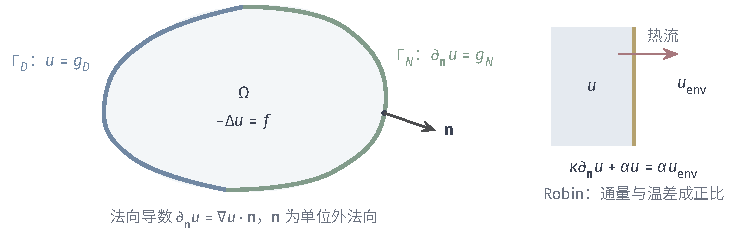
\includegraphics[width=124.5mm]{figures/03-optimization-evolution-and-signals/02-processes-and-trajectory-evolution/tikz/pde-domain-boundary/figure.pdf}
  \caption{区域与三类边界数据。左：区域$\Omega$内满足$-\Delta u=f$，边界的蓝色部分$\Gamma_D$规定场值，绿色部分$\Gamma_N$规定法向导数，箭头为一点处的单位外法向$\bm n$。右：Robin条件的物理来源，边界向外的热流与边界温度和环境温度之差成正比，系数$\alpha\geq0$。}
  \label{fig:pde-domain-boundary}
\end{figure*}

边界条件不是附加的细节，它改变解本身。下面的例子用同一个方程和同一个右端点条件，只改变左端点的类型。

\begin{example}[左端点的三种边界条件]
\label{ex:pde-three-boundary-conditions}
在$(0,1)$上考虑稳态热方程$-u''=1$，即棒内有均匀热源；右端$u(1)=0$。方程的通解是$u(x)=-x^2/2+Ax+B$。左端点的外法向指向$-x$方向，所以$\partial_{\bm n}u(0)=-u'(0)$。
\begin{itemize}
  \item Dirichlet条件$u(0)=0$：由$B=0$与$-\tfrac12+A=0$得$u(x)=x(1-x)/2$，最高温$1/8$在中点。
  \item Neumann条件$u'(0)=0$（左端绝热）：$A=0$，$B=\tfrac12$，$u(x)=(1-x^2)/2$，最高温$1/2$在绝热端。
  \item Robin条件$-u'(0)+\alpha u(0)=0$（取$\kappa=1$、$u_{\mathrm{env}}=0$）：$A=\alpha B$，再由$u(1)=0$得$B=1/(2(1+\alpha))$。取$\alpha=2$，$u(x)=-x^2/2+x/3+1/6$，左端温度$1/6$。
\end{itemize}
$\alpha=0$时Robin条件退化为Neumann条件；令$\alpha\to\infty$，$B\to0$、$A\to\tfrac12$，解趋于Dirichlet情形。
\end{example}

图~\ref{fig:pde-boundary-conditions}画出了这三条曲线。虚线是左端点的切线：Dirichlet曲线被钉在零点，Neumann曲线在左端水平，Robin曲线的左端斜率是左端值的两倍。热源相同，左端越“漏热”，整根棒越凉。

\begin{figure}[!htb]
  \centering
  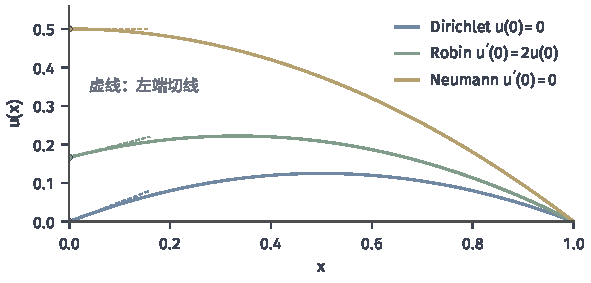
\includegraphics[width=100mm]{figures/03-optimization-evolution-and-signals/02-processes-and-trajectory-evolution/matplotlib/pde-boundary-conditions/figure.pdf}
  \caption{同一方程$-u''=1$、同一右端条件$u(1)=0$下，左端点取三种边界条件得到的解（例~\ref{ex:pde-three-boundary-conditions}）。圆点是左端值，虚线是左端切线：Dirichlet固定值为零，Neumann固定斜率为零，Robin条件$u'(0)=2u(0)$让斜率与值成比例。}
  \label{fig:pde-boundary-conditions}
\end{figure}

\paragraph{初值与边界在交接处的相容}
演化问题同时有初值和边界值，二者在区域边界与初始时刻的交接处相遇。回到细棒：若两端保持零度，而初始温度在整根棒上都是$1$，那么在角点$(x,t)=(0,0)$附近，沿$t=0$趋近得到$1$，沿$x=0$趋近得到$0$，解不可能在角点连续。第~\ref{sec:pde-heat-modes}小节会看到，这个问题对$t>0$仍有光滑的解，只是初值只能在平均意义下取到。

要让解在角点连续，至少需要\term{相容条件}（compatibility condition）$u_0(0)=g(0)$，即初值在边界上的取值与边界数据在初始时刻一致。更高的光滑性要求更多条件。例如对两端为零的热方程，边界上恒有$u=0$，于是边界上$u_t=0$；若希望$u_t$也连续到角点，方程$u_t=u_{xx}$还要求$u_0''(0)=u_0''(1)=0$。相容条件不满足时问题仍可能有解，但不连续性会从角点出发留在解中，对输运和波动方程尤其如此，它会沿着传播方向被带进区域内部。

\paragraph{经典解及其局限}
最直接的解释是逐点满足方程。对Poisson方程$-\Delta u=f$配零Dirichlet数据，\term{经典解}（classical solution）指$u\in C^2(\Omega)\cap C(\overline\Omega)$，在$\Omega$内每一点$-\Delta u=f$，在$\partial\Omega$上每一点$u=0$。这个要求在许多正常的问题上过强。

在$(0,1)$上取热源$f=2\cdot\mathbf 1_{[1/4,3/4]}$，只在中间一段加热。若$u$是经典解，则$u''=-f$在$x=1/4$两侧分别为$0$与$-2$，二阶导数不可能连续，所以经典解不存在。可是物理上应当有稳态温度：第~\ref{sec:pde-weak-form}小节将算出一个连续可微的$u$，它在除$x=1/4,3/4$外处处满足方程，跳跃只出现在二阶导数中。源集中在一点时情况更极端，一点处的点热源让温度曲线出现尖点，连一阶导数都在该点不存在。我们需要一种不要求逐点二阶导数的解释。

\paragraph{所用的Sobolev空间工具}
弱导数正是为此准备的工具。下面集中回顾本章要用的结论，它们都在固定开集$\Omega\subset\mathbb R^d$与Lebesgue测度下成立，$\langle u,v\rangle=\int_\Omega uv\,\mathrm d\bm x$与$\|u\|$分别表示$L^2(\Omega)$的内积与范数。
\begin{itemize}
  \item 若存在$v\in L^1_{\mathrm{loc}}(\Omega)$，使$\int_\Omega u\,\partial_i\varphi\,\mathrm d\bm x=-\int_\Omega v\varphi\,\mathrm d\bm x$对所有\term{测试函数}（test function）$\varphi\in C_c^\infty(\Omega)$成立，称$v$为$u$的弱导数$\partial_iu$；它在几乎处处意义下唯一。测试函数是在$\Omega$内某个紧集外为零的光滑函数，两个局部可积函数若与所有测试函数的积分都相同，则几乎处处相等。
  \item $H^1(\Omega)$由$u\in L^2(\Omega)$且各弱导数$\partial_iu\in L^2(\Omega)$的函数组成，内积$\langle u,v\rangle_{H^1}=\langle u,v\rangle+\int_\Omega\nabla u\cdot\nabla v\,\mathrm d\bm x$使它成为Hilbert空间。一维时，$H^1(a,b)$的每个元素有绝对连续的代表，满足$u(x)-u(y)=\int_y^xu'(s)\,\mathrm ds$，从而$|u(x)-u(y)|\leq|x-y|^{1/2}\|u'\|$。
  \item 设$\Omega$为有界Lipschitz区域。存在唯一的有界线性迹算子$\operatorname{Tr}:H^1(\Omega)\to L^2(\partial\Omega)$，在光滑到边界的函数上等于边界限制。$H_0^1(\Omega)$定义为$C_c^\infty(\Omega)$在$H^1$范数下的闭包，它恰好是迹为零的函数全体。若$g=\operatorname{Tr}G$，$G\in H^1(\Omega)$，则迹等于$g$的函数组成仿射集合$G+H_0^1(\Omega)$。
  \item Poincaré不等式：$\Omega$有界时，存在$C_P$使$\|u\|\leq C_P\|\nabla u\|$对所有$u\in H_0^1(\Omega)$成立；$\Omega$为有界连通Lipschitz区域时，存在$C$使$\|u-u_\Omega\|\leq C\|\nabla u\|$对所有$u\in H^1(\Omega)$成立，$u_\Omega$为均值。在区间$(0,L)$上两种情形的最优常数都是$L/\pi$。
  \item 紧嵌入：$\Omega$为有界Lipschitz区域时，$H^1(\Omega)$中的有界序列有在$L^2(\Omega)$中收敛的子列。
\end{itemize}
这些定义与定理的证明可参考\BookChapterRef{chap:weak-derivatives-sobolev}{卷二“弱导数与Sobolev空间”章}。本章用它们回答三件事：弱导数让“满足方程”可以通过与测试函数的积分来检验；迹让边界条件对$H^1$函数有意义；Poincaré不等式让梯度单独控制函数，这是后面能量估计的关键一步。

\paragraph{问题由数据、解空间与方程解释共同确定}
到这里可以说清一个偏微分方程问题由什么组成：区域与方程；源项、边界数据和初值，以及它们所属的函数空间；解所属的函数空间；“满足方程”的解释方式。后面将遇到三种解释：经典解逐点满足方程；\term{弱解}（weak solution）只要求与测试函数的积分关系成立，第~\ref{sec:pde-poisson}节为Poisson方程建立它；\term{温和解}（mild solution）用解算子与源项的积分公式定义演化，第~\ref{sec:pde-heat-semigroup}小节为热方程建立它。光滑性足够时三者一致，数据粗糙时只有较弱的解释可用。

选定这些空间以后，Hadamard提出的要求是：解存在，解唯一，并且解连续地依赖于数据，即数据的小扰动在所选范数下只引起解的小变化。三条都成立的问题称为\term{适定的}（well-posed）。三条要求都相对于所选空间而言：同一个热方程正向求解是适定的，反向求解（由今天的温度推算昨天的温度）在常用范数下却不满足连续依赖，第~\ref{sec:pde-heat-long-time}小节会给出具体的放大倍数。只写一条微分表达式，不交代数据、解空间和解释方式，问题还没有被确定。

% 第3章第2节：Poisson方程与弱解（从边值问题到弱形式；存在唯一与能量估计；其他边界条件与非唯一性）。

\section{Poisson方程与弱解}
\label{sec:pde-poisson}

本节研究不随时间变化的场。稳态温度、静电势、受载薄膜的位移都满足\term{Poisson方程}（Poisson equation）$-\Delta u=f$，其中$f$是源项。我们借这个方程完整走一遍三步：先把它改写成用测试函数检验的弱形式，再证明弱解存在唯一并用数据控制解，最后看边界条件改变时这些结论怎样随之改变。后面的热方程、波动方程和有限元方法都会沿用这里的弱形式与能量估计。

\subsection{从边值问题到弱形式}
\label{sec:pde-weak-form}

\paragraph{一维边值问题与Green函数}
先看能直接求解的情形：在$(0,1)$上求$u$，使
\begin{equation}
  -u''=f\quad\text{于}(0,1),\qquad u(0)=u(1)=0 .
  \label{eq:pde-poisson-1d}
\end{equation}
它描述两端固定、受分布载荷$f$的弦的平衡位移，也描述两端保持零度、有热源$f$的棒的稳态温度。对连续的$f$，积分两次并用边界条件定常数，可以把解写成
\begin{equation}
  u(x)=\int_0^1G(x,y)f(y)\,\mathrm dy,\qquad
  G(x,y)=\begin{cases}x(1-y),&0\leq x\leq y,\\ y(1-x),&y\leq x\leq1 .\end{cases}
  \label{eq:pde-green-1d}
\end{equation}
直接验证：$u(x)=(1-x)\int_0^xyf(y)\,\mathrm dy+x\int_x^1(1-y)f(y)\,\mathrm dy$，求导时两处边界项$\pm x(1-x)f(x)$互相抵消，得$u'(x)=-\int_0^xyf(y)\,\mathrm dy+\int_x^1(1-y)f(y)\,\mathrm dy$，再求导得$u''(x)=-xf(x)-(1-x)f(x)=-f(x)$；又$u(0)=u(1)=0$。函数$G$称为这个边值问题的\term{Green函数}（Green's function）。

$G(\cdot,y)$本身有清楚的含义：它是在$y$处放一个单位点热源时的稳态温度，形状是在$y$处取得最大值$y(1-y)$的“帐篷”。式~\eqref{eq:pde-green-1d}说，分布热源产生的温度是各点点源效应的叠加。图~\ref{fig:pde-poisson-energy}(a)画出三种总热量都为$1$的源：均匀源$f=1$给出$u=x(1-x)/2$，最高温$1/8$；只加热中段的$f=2\cdot\mathbf 1_{[1/4,3/4]}$给出最高温$3/16$；集中在中点的点源给出帐篷$G(\cdot,1/2)$，最高温$1/4$。热量越集中，中点越热。

式~\eqref{eq:pde-green-1d}的右端只需要$f$可积就有意义。对$f=2\cdot\mathbf 1_{[1/4,3/4]}$，上面$u'$的表达式仍然成立且连续，$u''=-f$在除$x=1/4,3/4$两点外成立。上一节已经说明这样的$u$不是经典解；点源的帐篷在$x=1/2$处连一阶导数都没有。这些物理上合理的“解”都需要一种新的检验方式。

\paragraph{用测试函数检验方程}
设$u$是式~\eqref{eq:pde-poisson-1d}的经典解，$\varphi\in C_c^\infty(0,1)$是测试函数。两边乘以$\varphi$再积分，用分部积分把一个导数从$u$移到$\varphi$上：
\[
  \int_0^1f\varphi\,\mathrm dx=-\int_0^1u''\varphi\,\mathrm dx
  =\int_0^1u'\varphi'\,\mathrm dx-\bigl[u'\varphi\bigr]_0^1
  =\int_0^1u'\varphi'\,\mathrm dx .
\]
边界项消失，因为$\varphi$在两端附近为零。右端只用到$u$的一阶导数，而$u$的二阶导数已经转移给了光滑的$\varphi$。

不妨把$\varphi$想成一个探针：把它放在某处，读出方程两边在这一小段上的加权平均。经典解要求方程在每一点成立；弱的检验只要求每一个探针读到的两个平均值相等。探针足够多时，这两种要求并不矛盾，因为与所有测试函数积分都相同的两个局部可积函数几乎处处相等。图~\ref{fig:pde-weak-form-test}用一个带尖点的函数说明这种转移：$u=\tfrac12-|x-\tfrac12|$在$x=1/2$处没有经典导数，弱导数$u'$是一个跳跃的阶梯；$u'\varphi$与$-u\varphi'$是两个完全不同的函数，积分却相等，都约为$-0.040$。

\begin{figure}[!htb]
  \centering
  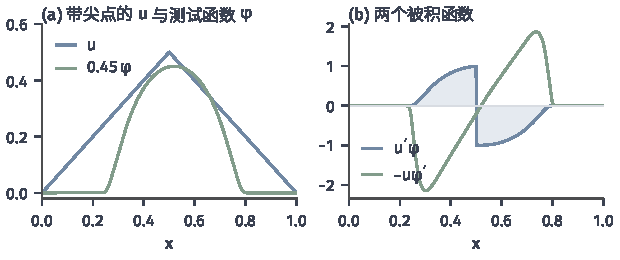
\includegraphics[width=105mm]{figures/03-optimization-evolution-and-signals/02-processes-and-trajectory-evolution/matplotlib/pde-weak-form-test/figure.pdf}
  \caption{把导数转移到测试函数上。(a)~$u=\tfrac12-|x-\tfrac12|$在$x=1/2$处有尖点；测试函数$\varphi$光滑，只在$(0.22,0.82)$内非零，图中缩小为$0.45$倍。(b)~两个被积函数：$u'\varphi$在尖点处跳跃（阴影），$-u\varphi'$连续；二者的积分在数值上都约为$-0.040$（梯形求积，$40001$个点）。}
  \label{fig:pde-weak-form-test}
\end{figure}

在$d$维有界区域上做同样的事，需要多元的分部积分。对向量场$v\nabla u$用散度定理，并利用$\nabla\cdot(v\nabla u)=\nabla v\cdot\nabla u+v\Delta u$，得到\term{Green第一恒等式}（Green's first identity）
\begin{equation}
  \int_\Omega(-\Delta u)\,v\,\mathrm d\bm x
  =\int_\Omega\nabla u\cdot\nabla v\,\mathrm d\bm x-\int_{\partial\Omega}(\partial_{\bm n}u)\,v\,\mathrm dS,
  \label{eq:pde-green-identity}
\end{equation}
它对有界Lipschitz区域、$u\in C^2(\overline\Omega)$与$v\in C^1(\overline\Omega)$成立。光滑边界上的散度定理（Gauss公式）及Laplace算子可参考\BookChapterRef{chap:multivariate-integration}{卷一“多元函数积分”章}；推广到Lipschitz边界需要几乎处处存在的外法向，这里不加证明地使用。若$v$在边界上为零，边界项消失，左边的二阶导数就变成了右边两个一阶导数的配对。

\paragraph{弱形式的定义}
式~\eqref{eq:pde-green-identity}提示：零Dirichlet边界的Poisson问题应当在$H_0^1(\Omega)$中寻找解，并用$H_0^1(\Omega)$中的函数检验。源项则只需要作为$H_0^1(\Omega)$上的连续线性泛函出现。由Poincaré不等式，$\|\nabla v\|$在$H_0^1(\Omega)$上与$H^1$范数等价，我们取它为$H_0^1(\Omega)$的范数，并把$H_0^1(\Omega)$上全体有界线性泛函组成的空间记为$H^{-1}(\Omega)$，范数为
\[
  \|\ell\|_{H^{-1}}=\sup_{v\in H_0^1(\Omega),\,v\neq0}\frac{|\ell(v)|}{\|\nabla v\|} .
\]

\begin{definition}[零Dirichlet边界Poisson问题的弱解]
\label{def:pde-weak-dirichlet}
设$\Omega\subset\mathbb R^d$为有界开集，$\ell\in H^{-1}(\Omega)$。若$u\in H_0^1(\Omega)$满足
\begin{equation}
  a(u,v):=\int_\Omega\nabla u\cdot\nabla v\,\mathrm d\bm x=\ell(v)\qquad\text{对所有}v\in H_0^1(\Omega),
  \label{eq:pde-weak-dirichlet}
\end{equation}
称$u$为$-\Delta u=\ell$在零Dirichlet边界条件下的弱解。$\ell(v)=\langle f,v\rangle$、$f\in L^2(\Omega)$时，也说$u$是$-\Delta u=f$的弱解。式~\eqref{eq:pde-weak-dirichlet}称为问题的\term{弱形式}（weak formulation）。
\end{definition}

定义里有三个选择，各有理由。第一，边界条件写进了解空间：$u\in H_0^1(\Omega)$在Lipschitz区域上就是迹为零。第二，检验函数取整个$H_0^1(\Omega)$而不只是$C_c^\infty(\Omega)$：两边对$v$都在$H^1$范数下连续，而$C_c^\infty(\Omega)$按定义在$H_0^1(\Omega)$中稠密，所以对测试函数成立等价于对全体$H_0^1$函数成立；扩大检验范围是为了下面能取$v=u$。第三，$f\in L^2(\Omega)$确实给出$H^{-1}$中的元素：由Cauchy--Schwarz与Poincaré不等式，
\[
  |\langle f,v\rangle|\leq\|f\|\,\|v\|\leq C_P\|f\|\,\|\nabla v\|,\qquad\text{故}\quad\|f\|_{H^{-1}}\leq C_P\|f\| .
\]

\begin{example}[一维点源是$H^{-1}$中的元素]
\label{ex:pde-point-source}
在$(0,1)$上固定$y$，令$\ell(v)=v(y)$，即点源只读取$v$在$y$处的值。$H_0^1(0,1)$的函数有连续代表且$v(0)=0$，所以$|v(y)|=|\int_0^yv'|\leq\sqrt y\,\|v'\|$，$\ell$有界，$\|\ell\|_{H^{-1}}\leq\sqrt y$。Green函数$u=G(\cdot,y)$就是对应的弱解：$G(\cdot,y)$在$(0,y)$上斜率为$1-y$，在$(y,1)$上斜率为$-y$，于是对任意$v\in H_0^1(0,1)$，
\[
  \int_0^1G_x(x,y)v'(x)\,\mathrm dx=(1-y)\bigl(v(y)-v(0)\bigr)-y\bigl(v(1)-v(y)\bigr)=v(y) .
\]
在$d\geq2$时情形不同：$H^1$函数可以在一点附近无界，读取点值不是$H_0^1$上的有界泛函，点源不属于$H^{-1}(\Omega)$，需要另外的解释。
\end{example}

\paragraph{经典解与弱解的关系}
弱解是经典解的推广，而不是另一个问题。下面的结论说明，在光滑的情形两种解释给出同一个对象。

\begin{theorem}[经典解与弱解]
\label{thm:pde-classical-weak}
设$\Omega$为有界Lipschitz区域，$f\in C(\overline\Omega)$。
\begin{enumerate}
  \item 若$u\in C^2(\overline\Omega)$在$\Omega$内满足$-\Delta u=f$，在$\partial\Omega$上$u=0$，则$u$是定义~\ref{def:pde-weak-dirichlet}意义下的弱解。
  \item 若弱解$u$还属于$C^2(\overline\Omega)$，则它在$\Omega$内处处满足$-\Delta u=f$，在$\partial\Omega$上处处为零。
\end{enumerate}
\end{theorem}

\begin{proof}
(1)~$u\in C^1(\overline\Omega)$，所以$u\in H^1(\Omega)$，其迹等于边界限制，为零；由零迹刻画，$u\in H_0^1(\Omega)$。对$v\in C_c^\infty(\Omega)$，式~\eqref{eq:pde-green-identity}的边界项为零，得$a(u,v)=\langle f,v\rangle$。两边对$v$在$H^1$范数下连续，由稠密性推广到全部$v\in H_0^1(\Omega)$。

(2)~对$\varphi\in C_c^\infty(\Omega)$，由式~\eqref{eq:pde-green-identity}与弱形式，$\int_\Omega(-\Delta u-f)\varphi\,\mathrm d\bm x=a(u,\varphi)-\langle f,\varphi\rangle=0$。连续函数$-\Delta u-f$与所有测试函数的积分为零，几乎处处为零，由连续性处处为零。又$u\in C^1(\overline\Omega)$时迹就是边界限制，而$u\in H_0^1(\Omega)$的迹为零，所以$u$在$\partial\Omega$上为零。
\end{proof}

\paragraph{与能量极小的对应}
弱形式还有一个能量的读法。定义
\begin{equation}
  J(v)=\frac12\int_\Omega|\nabla v|^2\,\mathrm d\bm x-\ell(v),\qquad v\in H_0^1(\Omega).
  \label{eq:pde-dirichlet-energy}
\end{equation}
对弦来说，第一项是拉伸储存的弹性能，第二项是载荷所做的功。展开平方，对任意$u,w\in H_0^1(\Omega)$，
\begin{equation}
  J(u+w)=J(u)+\bigl[a(u,w)-\ell(w)\bigr]+\frac12\|\nabla w\|^2 .
  \label{eq:pde-energy-expansion}
\end{equation}
若$u$是弱解，方括号对所有$w$为零，于是$J(u+w)=J(u)+\tfrac12\|\nabla w\|^2$；由Poincaré不等式，$\|\nabla w\|=0$迫使$w=0$，所以$u$是$J$的唯一最小点。反过来，若$u$最小化$J$，则一元二次函数$s\mapsto J(u+sw)$在$s=0$处取最小值，它在$s=0$处的导数正是方括号，必须为零，这就是弱形式。所以对这个对称问题，“弱解”与“能量最小点”是同一件事；弱形式是能量的一阶条件，在函数层面写出来就是$J$的\term{Euler--Lagrange方程}（Euler--Lagrange equation）。

图~\ref{fig:pde-poisson-energy}(b)沿两个方向画出了$f=1$时的$J(u+sw)$：每条都是开口向上的抛物线，最低点都在$s=0$，最低值都是$J(u)=-1/24$。曲率是$\|\nabla w\|^2$，$w=\sin(3\pi x)$的曲率是$w=\sin(\pi x)$的$9$倍，振荡越快的扰动付出的弹性能越大。

\begin{figure}[!htb]
  \centering
  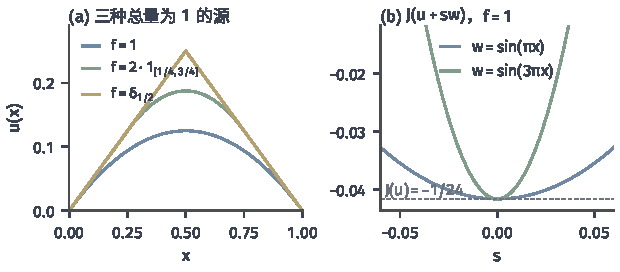
\includegraphics[width=105mm]{figures/03-optimization-evolution-and-signals/02-processes-and-trajectory-evolution/matplotlib/pde-poisson-energy/figure.pdf}
  \caption{一维Poisson问题~\eqref{eq:pde-poisson-1d}。(a)~三种总量为$1$的源对应的解：均匀源、中段加热与中点的点源，由Green函数~\eqref{eq:pde-green-1d}计算，最高值分别为$1/8$、$3/16$、$1/4$。(b)~$f=1$时能量~\eqref{eq:pde-dirichlet-energy}沿两个方向的截面$J(u+sw)=-\tfrac1{24}+\tfrac{s^2}{2}\|w'\|^2$，最小点都在$s=0$。}
  \label{fig:pde-poisson-energy}
\end{figure}

第~\ref{chap:optimization}章在有限维中证明过：可微凸函数的驻点就是全局最小点，强凸时最小点唯一。$J$是Hilbert空间上的二次凸函数，上面的展开是同一个结构的直接计算。可是有限维中证明最小点\emph{存在}所用的论证，即下水平集有界闭从而紧，在$H_0^1(\Omega)$中失效：无限维空间的有界闭集一般不紧。写出Euler--Lagrange方程只说明“如果有最小点，它满足什么”，并没有证明最小点或弱解存在，也没有说明数据怎样控制解。下一小节回答这两个问题。

\subsection{存在唯一与能量估计}
\label{sec:pde-lax-milgram}

\paragraph{双线性型与强制性}
把弱形式~\eqref{eq:pde-weak-dirichlet}抽象出来：$V$是实Hilbert空间，范数$\|\cdot\|_V$；$a:V\times V\to\mathbb R$对每个变量都是线性的，称为\term{双线性型}（bilinear form）；$\ell\in V'$是有界线性泛函。我们要求$u\in V$，使$a(u,v)=\ell(v)$对所有$v\in V$成立。两个条件将起关键作用：
\begin{equation}
  |a(u,v)|\leq M\|u\|_V\|v\|_V,\qquad a(v,v)\geq\alpha\|v\|_V^2,\qquad u,v\in V,
  \label{eq:pde-bounded-coercive}
\end{equation}
其中$M,\alpha>0$为常数。前者是有界性，后者称为$a$的\term{强制性}（coercivity）。在$V=\mathbb R^n$中，$a(u,v)=\bm v^{\top}\bm K\bm u$，强制性就是$\bm v^{\top}\bm K\bm v\geq\alpha\|\bm v\|_2^2$：沿任何方向推动，$a$都给出与推动量平方成比例的正回应。这样的矩阵没有非零零向量，因而可逆。下面要在无限维中得到同样的结论。

\paragraph{对称情形：Riesz表示}
若$a$还是对称的，$a(u,v)=a(v,u)$，则$(u,v)_a:=a(u,v)$是$V$上的内积。式~\eqref{eq:pde-bounded-coercive}给出$\alpha\|v\|_V^2\leq(v,v)_a\leq M\|v\|_V^2$，新范数与原范数等价，所以$V$在新内积下仍完备，$\ell$在新范数下仍有界。Hilbert空间上的Riesz表示定理说：每个有界线性泛函$\ell$都等于与某个唯一元素的内积，并且这个元素的范数等于$\ell$的范数，可参考\BookChapterRef{chap:linear-functionals-operators}{卷二“线性泛函与线性算子”章}。对内积$(\cdot,\cdot)_a$使用它，立即得到唯一的$u$满足$(u,v)_a=\ell(v)$。Poisson方程正是这种情形：取$V=H_0^1(\Omega)$、内积$(u,v)_a=\int_\Omega\nabla u\cdot\nabla v$，Poincaré不等式保证它与$H^1$内积等价。

\paragraph{Lax--Milgram定理}
对流、Robin边界等问题给出不对称的或带边界项的双线性型，需要不依赖对称性的结论。

\begin{theorem}[Lax--Milgram定理]
\label{thm:pde-lax-milgram}
设$V$为实Hilbert空间，双线性型$a$满足有界性与强制性~\eqref{eq:pde-bounded-coercive}，$\ell\in V'$。则存在唯一的$u\in V$，使$a(u,v)=\ell(v)$对所有$v\in V$成立，并且$\|u\|_V\leq\|\ell\|_{V'}/\alpha$。
\end{theorem}

\begin{proof}
第一步，把$a$表示成算子。对固定的$u$，$v\mapsto a(u,v)$是$V$上的有界线性泛函，由Riesz表示存在唯一的$Au\in V$，使$\langle Au,v\rangle_V=a(u,v)$对所有$v$成立。$A$是线性的，且$\|Au\|_V\leq M\|u\|_V$。同理取$r\in V$使$\ell(v)=\langle r,v\rangle_V$。问题化为解$Au=r$。

第二步，$A$有下界。由强制性与Cauchy--Schwarz不等式，$\alpha\|u\|_V^2\leq a(u,u)=\langle Au,u\rangle_V\leq\|Au\|_V\|u\|_V$，所以$\|Au\|_V\geq\alpha\|u\|_V$。于是$A$是单射；值域闭：若$Au_n\to w$，则$\|u_n-u_m\|_V\leq\alpha^{-1}\|Au_n-Au_m\|_V$说明$(u_n)$是Cauchy列，收敛到某个$u$，由$A$连续得$Au=w$。

第三步，值域是全空间。若$w$与$A$的值域正交，则$0=\langle Aw,w\rangle_V=a(w,w)\geq\alpha\|w\|_V^2$，$w=0$。闭子空间的正交补为零，它就是全空间。所以存在唯一的$u$使$Au=r$。最后，$\alpha\|u\|_V^2\leq a(u,u)=\ell(u)\leq\|\ell\|_{V'}\|u\|_V$，给出范数界。
\end{proof}

定理的结论包括了连续依赖：两组数据$\ell_1,\ell_2$对应的解之差满足同一问题，右端为$\ell_1-\ell_2$，所以$\|u_1-u_2\|_V\leq\|\ell_1-\ell_2\|_{V'}/\alpha$。强制常数$\alpha$越小，数据扰动被放大得越厉害。

\begin{example}[不对称的对流扩散问题]
\label{ex:pde-convection-diffusion}
在$(0,1)$上考虑$-u''+\beta u'=f$，$u(0)=u(1)=0$，$\beta$为常数，$\beta u'$表示以速度$\beta$流动的介质把热量向下游带。弱形式为$a(u,v)=\int_0^1(u'v'+\beta u'v)\,\mathrm dx=\langle f,v\rangle$，$a$不对称。可是对$v\in H_0^1(0,1)$，$\int_0^1v'v\,\mathrm dx=\tfrac12[v^2]_0^1=0$，所以$a(v,v)=\|v'\|^2$，强制常数与$\beta$无关；有界性由$|\int\beta u'v|\leq|\beta|\,\|u'\|\,\|v\|\leq|\beta|C_P\|u'\|\,\|v'\|$得到。由定理~\ref{thm:pde-lax-milgram}，对任意$\beta$与$f\in L^2$，弱解存在唯一。这里不能用Riesz表示直接求解，因为$a$不是内积。
\end{example}

\paragraph{Poisson方程的弱解存在唯一}
把定理~\ref{thm:pde-lax-milgram}用到定义~\ref{def:pde-weak-dirichlet}，得到本节的主要结论。

\begin{theorem}[Dirichlet问题的弱解]
\label{thm:pde-dirichlet-existence}
设$\Omega\subset\mathbb R^d$为有界开集，$C_P$为Poincaré常数。对每个$\ell\in H^{-1}(\Omega)$，零Dirichlet边界的Poisson问题有唯一弱解$u\in H_0^1(\Omega)$，且$\|\nabla u\|\leq\|\ell\|_{H^{-1}}$。若$\ell=\langle f,\cdot\rangle$，$f\in L^2(\Omega)$，则
\begin{equation}
  \|\nabla u\|\leq C_P\|f\|,\qquad\|u\|\leq C_P^2\|f\| .
  \label{eq:pde-poisson-energy-estimate}
\end{equation}
\end{theorem}

\begin{proof}
取$V=H_0^1(\Omega)$，范数$\|\nabla v\|$。它与$H^1$范数等价，而$H_0^1(\Omega)$是$H^1(\Omega)$的闭子空间，所以$V$是Hilbert空间。$a(u,v)=\int\nabla u\cdot\nabla v$就是这个内积，$M=\alpha=1$，定理~\ref{thm:pde-lax-milgram}给出存在唯一与$\|\nabla u\|\leq\|\ell\|_{H^{-1}}$。对$f\in L^2$，在弱形式中取$v=u$，得$\|\nabla u\|^2=\langle f,u\rangle\leq\|f\|\,\|u\|\leq C_P\|f\|\,\|\nabla u\|$，约去$\|\nabla u\|$得第一式；再用一次Poincaré不等式得第二式。
\end{proof}

这个定理只要求$\Omega$有界，不要求边界规则；只有当我们想把$u\in H_0^1(\Omega)$解释成“迹为零”或处理非零边界数据时，才需要Lipschitz边界。

\paragraph{能量估计与连续依赖}
上面证明中“取$v=u$”的一步称为\term{能量估计}（energy estimate），这个技巧在本章反复出现：用解本身检验方程，左边变成某种能量，右边用数据控制。由于问题是线性的，两组源项$f_1,f_2$的解之差$u_1-u_2$是源项$f_1-f_2$的弱解，于是$\|\nabla(u_1-u_2)\|\leq C_P\|f_1-f_2\|$：源项在$L^2$中的小扰动只引起解在能量范数下的小变化。

可以用$f=1$的例子核对估计~\eqref{eq:pde-poisson-energy-estimate}。在$(0,1)$上最优常数$C_P=1/\pi$，$\|f\|=1$。解$u=x(1-x)/2$满足$u'=\tfrac12-x$，$\|u'\|^2=\int_0^1(\tfrac12-x)^2\,\mathrm dx=\tfrac1{12}$，$\|u'\|\approx0.289\leq1/\pi\approx0.318$；又$\|u\|^2=\tfrac14\int_0^1x^2(1-x)^2\,\mathrm dx=\tfrac1{120}$，$\|u\|\approx0.091\leq1/\pi^2\approx0.101$。两个界都成立且相当接近，因为$f=1$在正弦展开中主要落在最低频的$\sin(\pi x)$方向上，而Poincaré不等式恰在这个方向上取等。

\paragraph{非齐次Dirichlet数据}
若边界上规定$u=g$，设$\Omega$为有界Lipschitz区域，$g=\operatorname{Tr}G$，$G\in H^1(\Omega)$。迹等于$g$的函数组成$G+H_0^1(\Omega)$，所以令$u=G+w$，$w\in H_0^1(\Omega)$满足
\[
  a(w,v)=\langle f,v\rangle-a(G,v)\qquad\text{对所有}v\in H_0^1(\Omega).
\]
右端对$v$有界，因为$|a(G,v)|\leq\|\nabla G\|\,\|\nabla v\|$，所以$w$存在唯一，$\|\nabla w\|\leq C_P\|f\|+\|\nabla G\|$。结果不依赖$G$的选取：两个延拓给出的$u$之差属于$H_0^1(\Omega)$且满足右端为零的问题，只能为零。估计$\|\nabla u\|\leq C_P\|f\|+2\|\nabla G\|$说明边界数据通过它的延拓被控制；对所有延拓取下确界得到边界数据的一个范数，它的精确刻画需要分数阶Sobolev空间，这里不展开。

\paragraph{弱解何时更光滑}
弱解只保证一个弱导数平方可积。数据和区域更好时，解可能更光滑，但这需要另外证明。一维情形可以完整做出来。

\begin{theorem}[一维弱解的正则性]
\label{thm:pde-regularity-1d}
设$f\in L^2(0,1)$，$u\in H_0^1(0,1)$是$-u''=f$的弱解。则$u'$属于$H^1(0,1)$且弱导数为$-f$；因而$u$有连续可微的代表，$u'$绝对连续，并且$-u''=f$几乎处处成立。
\end{theorem}

\begin{proof}
对$\varphi\in C_c^\infty(0,1)$，弱形式给出$\int_0^1u'\varphi'\,\mathrm dx=\int_0^1f\varphi\,\mathrm dx=-\int_0^1(-f)\varphi\,\mathrm dx$。按弱导数的定义，$u'$的弱导数是$-f\in L^2$，所以$u'\in H^1(0,1)$，它有绝对连续的代表。$u$是这个连续函数的不定积分，因而连续可微。
\end{proof}

高维情形结论依赖区域。可以证明：$f\in L^2(\Omega)$时弱解在每个内部紧集上属于$H^2$；若边界是$C^2$的或$\Omega$是凸的，则在整个$\Omega$上属于$H^2$。区域有向内凹的角时，整体结论可以失败。在L形区域的凹角处取极坐标$(r,\theta)$，函数$r^{2/3}\sin(2\theta/3)$在角的两条边上为零，满足$\Delta u=0$；它的梯度大小约为$r^{-1/3}$，平方可积，二阶导数大小约为$r^{-4/3}$，而$\int_0r^{-8/3}\,r\,\mathrm dr$发散，所以它不在凹角附近的$H^2$中。点源的帐篷函数也是例子：它属于$H^1$，导数在源点跳跃，不属于$H^2$。弱解存在不等于有逐点二阶导数。

\subsection{其他边界条件与非唯一性}
\label{sec:pde-other-boundary}

前两小节的结论都建立在零Dirichlet边界上：边界条件写进解空间，Poincaré不等式提供强制性。换成Neumann或Robin边界，这两步都要重新检查。

\paragraph{Neumann问题的弱形式}
设$\Omega$为有界连通Lipschitz区域，$f\in L^2(\Omega)$，$g\in L^2(\partial\Omega)$，考虑
\[
  -\Delta u=f\quad\text{于}\Omega,\qquad\partial_{\bm n}u=g\quad\text{于}\partial\Omega .
\]
这次边界上不规定$u$的值，所以检验函数也不必在边界上为零。在Green恒等式~\eqref{eq:pde-green-identity}中取一般的$v\in C^1(\overline\Omega)$，边界项不再消失，而是由数据$g$给出：
\begin{equation}
  \int_\Omega\nabla u\cdot\nabla v\,\mathrm d\bm x=\int_\Omega fv\,\mathrm d\bm x+\int_{\partial\Omega}g\operatorname{Tr}v\,\mathrm dS\qquad\text{对所有}v\in H^1(\Omega).
  \label{eq:pde-weak-neumann}
\end{equation}
称满足上式的$u\in H^1(\Omega)$为Neumann问题的弱解。右端对$v$有界，因为由迹定理$|\int_{\partial\Omega}g\operatorname{Tr}v|\leq\|g\|_{L^2(\partial\Omega)}C_{\mathrm{Tr}}\|v\|_{H^1}$。

与Dirichlet情形对照，边界条件进入问题的方式不同。Dirichlet条件写进解空间，称为\term{本质边界条件}（essential boundary condition）；Neumann条件没有出现在解空间中，而是藏在弱形式的边界积分里，称为\term{自然边界条件}（natural boundary condition）。若弱解足够光滑，先用$v\in C_c^\infty(\Omega)$检验得$-\Delta u=f$，再对一般的$v$比较式~\eqref{eq:pde-green-identity}与式~\eqref{eq:pde-weak-neumann}，得$\int_{\partial\Omega}(\partial_{\bm n}u-g)v\,\mathrm dS=0$；边界上的这些$v$足够多，于是$\partial_{\bm n}u=g$，边界条件被“自然地”恢复出来。

\paragraph{相容条件与常数方向}
在式~\eqref{eq:pde-weak-neumann}中取$v=1$，左边为零，得到
\begin{equation}
  \int_\Omega f\,\mathrm d\bm x+\int_{\partial\Omega}g\,\mathrm dS=0 .
  \label{eq:pde-neumann-compatibility}
\end{equation}
这是解存在的必要条件。按热传导的读法，$f$是区域内产生的热量，$g=\partial_{\bm n}u$是从边界流入的热量（向外热流为$-\partial_{\bm n}u$）。稳态意味着总热量不变，内部产生的与边界流入的总和必须为零。一维时，$-u''=f$配$u'(0)=u'(1)=0$要求$\int_0^1f=0$；$f=1$在两端绝热的棒中持续加热，不可能有稳态。

另一方面，若$u$是解，$u+c$对任何常数$c$也是解，因为常数的梯度为零。图~\ref{fig:pde-neumann}(a)画出了$-u''=\pi^2\cos(\pi x)$在两端绝热时的几个解$\cos(\pi x)+c$：源项均值为零，相容条件成立，但解只确定到相差一个常数。图~\ref{fig:pde-neumann}(b)则把相容条件不成立的情形放到时间中去看：源项均值为$1$时，温度剖面的形状趋于稳定，整体水平却按$t$线性上升，永远达不到稳态。

\begin{figure}[!htb]
  \centering
  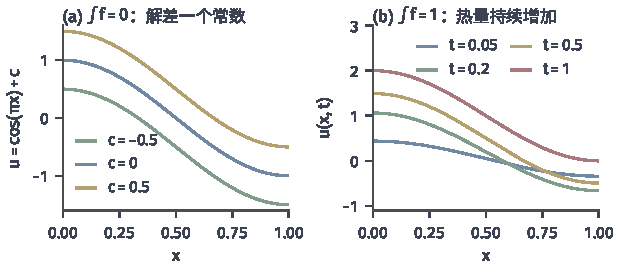
\includegraphics[width=105mm]{figures/03-optimization-evolution-and-signals/02-processes-and-trajectory-evolution/matplotlib/pde-neumann/figure.pdf}
  \caption{两端绝热的棒。(a)~$f=\pi^2\cos(\pi x)$满足相容条件$\int_0^1f=0$，$\cos(\pi x)+c$对每个常数$c$都是解。(b)~$f=1+\pi^2\cos(\pi x)$不满足相容条件；从零初温出发的热方程$u_t=u_{xx}+f$的解为$u=t+(1-e^{-\pi^2t})\cos(\pi x)$，形状趋于$\cos(\pi x)$，平均温度按$t$增长。}
  \label{fig:pde-neumann}
\end{figure}

\paragraph{零均值空间中的唯一解}
为了去掉常数方向，把解限制在均值为零的函数中，Poincaré不等式的零均值形式恰好提供所需的强制性。

\begin{theorem}[Neumann问题的弱解]
\label{thm:pde-neumann}
设$\Omega$为有界连通Lipschitz区域，$f\in L^2(\Omega)$，$g\in L^2(\partial\Omega)$。Neumann问题~\eqref{eq:pde-weak-neumann}有弱解当且仅当相容条件~\eqref{eq:pde-neumann-compatibility}成立；此时弱解在相差常数的意义下唯一，在$V=\{v\in H^1(\Omega):\int_\Omega v\,\mathrm d\bm x=0\}$中恰有一个。
\end{theorem}

\begin{proof}
必要性已由$v=1$得到。设相容条件成立。$v\mapsto\int_\Omega v$在$H^1$上连续，所以$V$是闭子空间，本身是Hilbert空间。对$v\in V$，零均值的Poincaré不等式给出$\|v\|\leq C\|\nabla v\|$，于是$\|v\|_{H^1}^2\leq(1+C^2)\|\nabla v\|^2=(1+C^2)a(v,v)$，$a$在$V$上强制。式~\eqref{eq:pde-weak-neumann}的右端$\ell$在$V$上有界，由定理~\ref{thm:pde-lax-milgram}存在唯一$u\in V$使$a(u,v)=\ell(v)$对$v\in V$成立。

还需验证对所有$v\in H^1(\Omega)$成立。把$v$写成$v=(v-v_\Omega)+v_\Omega$，第一项属于$V$；对常数$v_\Omega$，$a(u,v_\Omega)=0$，而$\ell(v_\Omega)=v_\Omega\bigl(\int_\Omega f+\int_{\partial\Omega}g\bigr)=0$正是相容条件。所以$u$是弱解。若$u_1,u_2$都是弱解，差$w$满足$a(w,w)=0$，$\nabla w=0$，在连通区域上$w$是常数。
\end{proof}

区域不连通时，每个连通分支都有自己的常数方向和自己的相容条件。定理中的连通性不能省略，与Poincaré不等式的零均值形式需要连通性是同一个原因。

\paragraph{Robin边界：边界项进入双线性型}
Robin条件$\partial_{\bm n}u+\alpha u=g$（取$\kappa=1$）把$\partial_{\bm n}u=g-\alpha u$代入Green恒等式的边界项，得到弱形式
\begin{equation}
  \begin{aligned}
    a_R(u,v)&:=\int_\Omega\nabla u\cdot\nabla v\,\mathrm d\bm x+\int_{\partial\Omega}\alpha\operatorname{Tr}u\operatorname{Tr}v\,\mathrm dS\\
    &=\int_\Omega fv\,\mathrm d\bm x+\int_{\partial\Omega}g\operatorname{Tr}v\,\mathrm dS,\qquad v\in H^1(\Omega).
  \end{aligned}
  \label{eq:pde-weak-robin}
\end{equation}
边界条件的一半进入了右端，另一半进入了双线性型。设$\alpha\in L^\infty(\partial\Omega)$，由迹定理$a_R$有界。强制性需要一个把边界值也算进来的不等式。

\begin{lemma}[带边界项的Poincaré型不等式]
\label{lem:pde-friedrichs}
设$\Omega$为有界连通Lipschitz区域。存在常数$C_F$，使所有$v\in H^1(\Omega)$满足$\|v\|^2\leq C_F\bigl(\|\nabla v\|^2+\|\operatorname{Tr}v\|_{L^2(\partial\Omega)}^2\bigr)$。
\end{lemma}

\begin{proof}
反设不成立，则有$v_n\in H^1(\Omega)$，$\|v_n\|=1$，而$\|\nabla v_n\|^2+\|\operatorname{Tr}v_n\|_{L^2(\partial\Omega)}^2<1/n$。序列在$H^1$中有界，由紧嵌入，有子列（仍记为$v_n$）在$L^2$中收敛到某个$v$，$\|v\|=1$。由于$\|v_n-v_m\|_{H^1}^2=\|v_n-v_m\|^2+\|\nabla v_n-\nabla v_m\|^2$且两项都趋于零，$(v_n)$在$H^1$中是Cauchy列，在$H^1$中收敛到$v$，$\nabla v=0$；区域连通，$v$几乎处处等于常数$c$，$|c|\,|\Omega|^{1/2}=1$。迹算子连续，$\operatorname{Tr}v_n\to\operatorname{Tr}v=c$，而$\|\operatorname{Tr}v_n\|\to0$，所以$c=0$，矛盾。
\end{proof}

若$\alpha\geq\alpha_0>0$几乎处处成立，则$a_R(v,v)\geq\min(1,\alpha_0)\bigl(\|\nabla v\|^2+\|\operatorname{Tr}v\|^2\bigr)$，由引理~\ref{lem:pde-friedrichs}，$\|v\|_{H^1}^2\leq(C_F+1)\bigl(\|\nabla v\|^2+\|\operatorname{Tr}v\|^2\bigr)$，所以$a_R$在整个$H^1(\Omega)$上强制。由定理~\ref{thm:pde-lax-milgram}，弱解存在唯一，不需要相容条件，也没有常数方向。物理上，边界只要有一点“漏热”，稳态就被唯一确定。

\paragraph{系数符号}
上面用到$\alpha\geq\alpha_0>0$。符号反过来，结论可以失效。在$(0,1)$上两端都取Robin条件，外法向在左端指向$-x$、在右端指向$+x$，条件为$-u'(0)+\alpha u(0)=0$与$u'(1)+\alpha u(1)=0$。对$-u''=0$，解为$u=A+Bx$，代入得$B=\alpha A$与$\alpha A(2+\alpha)=0$。$\alpha=-2$时$A$任意，$u=1-2x$是非零解，所以齐次问题有非零解，唯一性失败。这时$a_R(1,1)=\alpha\cdot(1+1)=-4<0$，强制性不成立。物理上$\alpha<0$意味着边界越热、从外界吸收的热量越多，这已不是Newton冷却。

\paragraph{三种边界条件的对照}
表~\ref{tab:pde-boundary-comparison}汇总了本小节的比较。同一个方程$-\Delta u=f$，边界条件一变，解空间、边界条件进入弱形式的位置、存在所需的条件以及唯一性都随之改变，不能把Dirichlet版本的结论直接搬过去。

\begin{table*}[!htb]
  \centering
  \begin{tabularx}{\linewidth}{@{}l>{\RaggedRight\arraybackslash}X>{\RaggedRight\arraybackslash}X>{\RaggedRight\arraybackslash}X@{}}
    \toprule
    边界条件 & 解空间 & 条件进入弱形式的位置 & 存在与唯一 \\
    \midrule
    Dirichlet $u=g$ & $G+H_0^1(\Omega)$ & 解空间（本质条件） & 总存在且唯一 \\
    Neumann $\partial_{\bm n}u=g$ & $H^1(\Omega)$ & 右端边界积分（自然条件） & 需相容条件，差常数 \\
    Robin $\partial_{\bm n}u+\alpha u=g$ & $H^1(\Omega)$ & 双线性型与右端 & 总存在且唯一 \\
    \bottomrule
  \end{tabularx}
  \caption{Poisson方程三种边界条件的弱形式对照（$\Omega$为有界连通Lipschitz区域，Robin情形设$\alpha\geq\alpha_0>0$）。}
  \label{tab:pde-boundary-comparison}
\end{table*}

% 第3章第3节：热方程与扩散（扩散方程与模式衰减；弱演化与解算子；能量、正性与长期极限）。

\section{热方程与扩散}
\label{sec:pde-heat}

上一节的场不随时间变化。本节让场动起来：热量从热处流向冷处，温度场随时间被抹平。我们先从守恒关系推出方程，用可以直接验证的正弦模式看清“高频衰减更快”；再在函数空间中建立弱解与解算子，把热方程放进与上一章矩阵指数平行的框架；最后研究能量、总热量、正性和长期极限。

\subsection{扩散方程与模式衰减}
\label{sec:pde-heat-modes}

\paragraph{从守恒与通量得到热方程}
回到细棒。设棒的密度为$\rho$、比热为$c$，截面积取为$1$，温度为$u(x,t)$。区间$[a,b]$中的热量是$\int_a^b\rho cu\,\mathrm dx$。记$q(x,t)$为单位时间内向右穿过截面$x$的热量，$s(x,t)$为单位长度的热源功率。热量守恒说：$[a,b]$中热量的变化率，等于从左端流入的、减去从右端流出的，再加上内部产生的，
\[
  \frac{\mathrm d}{\mathrm dt}\int_a^b\rho cu\,\mathrm dx=q(a,t)-q(b,t)+\int_a^bs\,\mathrm dx .
\]
这是一个积分形式的平衡，还没有说明热流由什么决定。\term{Fourier定律}（Fourier's law）补上这一步：热流与温度梯度成正比、方向相反，$q=-k\,u_x$，$k>0$为导热系数。热总是从热处流向冷处。

设各量足够光滑，把$q(a)-q(b)=-\int_a^bq_x\,\mathrm dx$代入，得$\int_a^b(\rho cu_t-(ku_x)_x-s)\,\mathrm dx=0$。它对所有$a<b$成立，被积函数又连续，只能处处为零。系数为常数时，令$\kappa=k/(\rho c)$、$f=s/(\rho c)$，得到\term{热方程}（heat equation）
\begin{equation}
  u_t=\kappa u_{xx}+f .
  \label{eq:pde-heat-1d}
\end{equation}
$\kappa$称为\term{扩散系数}（diffusion coefficient）。在$d$维区域中，同样的推理把端点通量换成穿过任意小区域边界的通量，用散度定理得到$u_t=\nabla\cdot(\kappa\nabla u)+f$，常系数时即$u_t=\kappa\Delta u+f$。边界上的热交换就是第~\ref{sec:pde-boundary-solution-meaning}小节的三类边界条件。

式~\eqref{eq:pde-neighbor-average}给出了这个方程的直观读法：$\kappa u_{xx}\approx(2\kappa/h^2)\bigl(\text{邻居平均值}-u\bigr)$。每一点都以正比于“自己与邻居之差”的速率向邻居的平均值靠拢，比邻居高的地方降温，比邻居低的地方升温。下面取$\kappa=1$；一般的$\kappa$只需把时间换成$\kappa t$。

\paragraph{正弦模式的指数衰减}
在$(0,1)$上取两端为零的Dirichlet条件，无源。不急于解一般的初值，先猜一个形状不变、只按比例缩小的解$u(x,t)=a(t)\sin(k\pi x)$，$k$为正整数。它满足两端为零；代入方程，$a'(t)\sin(k\pi x)=-k^2\pi^2a(t)\sin(k\pi x)$，所以$a(t)=a(0)e^{-k^2\pi^2t}$。

于是每个正弦形状都是一个\term{特征模式}（eigenmode）：它在演化中保持形状，振幅按$e^{-\lambda_kt}$衰减，衰减率$\lambda_k=k^2\pi^2$随频率的平方增长。振幅减半所需的时间是$\ln2/\lambda_k$：$k=1$时约为$0.070$，$k=4$时约为$0.0044$，相差$16$倍。原因在式~\eqref{eq:pde-neighbor-average}中：$\sin(k\pi x)$的曲率$k^2\pi^2\sin(k\pi x)$随频率平方增大，振荡越快，每个峰与邻居的落差相对越大，被抹平得越快。

\paragraph{叠加与高频更快衰减}
方程是线性的，模式可以叠加。图~\ref{fig:pde-heat-modes}(a)的初值是$\sin(\pi x)+\tfrac12\sin(4\pi x)$：高频的小起伏在$t=0.015$时已几乎看不见，剩下的是缓慢下降的最低模式；图~\ref{fig:pde-heat-modes}(b)在对数坐标中画出各模式的振幅，它们是斜率为$-k^2\pi^2$的直线。

\begin{figure}[!htb]
  \centering
  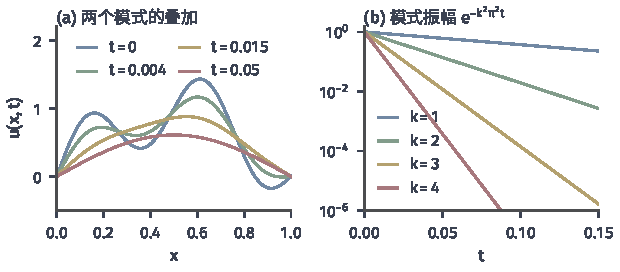
\includegraphics[width=105mm]{figures/03-optimization-evolution-and-signals/02-processes-and-trajectory-evolution/matplotlib/pde-heat-modes/figure.pdf}
  \caption{热方程$u_t=u_{xx}$在两端为零时的模式衰减。(a)~初值$\sin(\pi x)+\tfrac12\sin(4\pi x)$的解$e^{-\pi^2t}\sin(\pi x)+\tfrac12e^{-16\pi^2t}\sin(4\pi x)$在四个时刻的形状，高频起伏先消失。(b)~第$k$个模式的振幅$e^{-k^2\pi^2t}$，纵轴为对数刻度，斜率$-k^2\pi^2$。}
  \label{fig:pde-heat-modes}
\end{figure}

一般的初值能否写成这些模式的叠加？需要两件事：模式两两正交，并且足以表示$L^2(0,1)$中的每个函数。记$e_k(x)=\sqrt2\sin(k\pi x)$，直接积分可知$\langle e_j,e_k\rangle$在$j=k$时为$1$、否则为$0$。完备性来自Green函数。式~\eqref{eq:pde-green-1d}定义的积分算子$(\mathcal Gf)(x)=\int_0^1G(x,y)f(y)\,\mathrm dy$的核平方可积且对称，因而是$L^2(0,1)$上的紧自伴算子；由定理~\ref{thm:pde-regularity-1d}，$\mathcal Gf$是$-u''=f$的弱解，所以$\mathcal Gf=0$推出$f=-(\mathcal Gf)''=0$，$\mathcal G$是单射。若$\mathcal G\varphi=\mu\varphi$且$\mu\neq0$，则$\varphi=\mathcal G(\varphi/\mu)$满足$-\varphi''=\varphi/\mu$与两端为零，只能是$\sin(k\pi x)$的倍数，$\mu=1/(k^2\pi^2)$。紧自伴算子的谱分解说，非零特征值的特征向量组成核的正交补的标准正交基，可参考\BookChapterRef{chap:operator-spectra-equations}{卷二“算子谱与算子方程”章}；这里核为零，所以$\{e_k\}_{k\geq1}$是$L^2(0,1)$的标准正交基。

\begin{theorem}[区间上热方程的级数解]
\label{thm:pde-heat-series}
设$u_0\in L^2(0,1)$，$c_k=\langle u_0,e_k\rangle$。令
\begin{equation}
  u(t)=\sum_{k=1}^\infty c_ke^{-k^2\pi^2t}e_k,\qquad t\geq0 .
  \label{eq:pde-heat-series}
\end{equation}
则(1)对每个$t\geq0$，级数在$L^2(0,1)$中收敛，$\|u(t)\|\leq e^{-\pi^2t}\|u_0\|$，并且$t\to0^+$时$\|u(t)-u_0\|\to0$；(2)对每个$t_0>0$，级数及其关于$x$、$t$的逐项各阶导数在$[0,1]\times[t_0,\infty)$上一致收敛，所以$u$在$[0,1]\times(0,\infty)$上无穷次可微，经典地满足$u_t=u_{xx}$与$u(0,t)=u(1,t)=0$。
\end{theorem}

\begin{proof}
(1)~由Parseval等式$\sum_kc_k^2=\|u_0\|^2$，系数$c_ke^{-k^2\pi^2t}$平方可和，级数收敛，且$\|u(t)\|^2=\sum_kc_k^2e^{-2k^2\pi^2t}\leq e^{-2\pi^2t}\|u_0\|^2$。又$\|u(t)-u_0\|^2=\sum_kc_k^2(1-e^{-k^2\pi^2t})^2$，每一项随$t\to0^+$趋于零且不超过$c_k^2$，由控制收敛定理（对计数测度）趋于零。

(2)~$|c_k|\leq\|u_0\|$。对$x$求$m$阶、对$t$求$n$阶导数后，第$k$项的绝对值不超过$\sqrt2\|u_0\|(k\pi)^{m+2n}e^{-k^2\pi^2t_0}$，它关于$k$可和，因为$e^{-k^2\pi^2t_0}$比$k$的任何幂次衰减得都快。由Weierstrass判别法，各阶导数的级数一致收敛，可以逐项求导。每一项都满足方程与边界条件，所以和也满足。
\end{proof}

定理的(2)说出了扩散最重要的性质：无论初值多粗糙，只要它平方可积，解在任意正时刻都是光滑的。系数被$e^{-k^2\pi^2t}$压制，高频成分在瞬间就被抹去。称这一现象为热方程的\term{磨光效应}（smoothing effect）。

\paragraph{初值的光滑程度与解的意义}
取$u_0=1$，正是第~\ref{sec:pde-boundary-solution-meaning}小节讨论过的、与零边界不相容的初值。系数为$c_k=\sqrt2\int_0^1\sin(k\pi x)\,\mathrm dx=\sqrt2(1-\cos k\pi)/(k\pi)$，偶数$k$为零、奇数$k$为$2\sqrt2/(k\pi)$，所以
\[
  u(x,t)=\sum_{k\ \text{奇}}\frac{4}{k\pi}e^{-k^2\pi^2t}\sin(k\pi x).
\]
在$t=0$，这个级数在$L^2$中收敛到$1$，但不一致收敛：每个部分和在两端都等于零，而且项数增多时，部分和在端点附近的最高值趋于约$1.18$而不是$1$（Gibbs现象：奇延拓后端点处有高为$2$的跳跃，超出量约为跳跃的百分之九）。对$t>0$，定理~\ref{thm:pde-heat-series}保证解光滑并在两端为零。所以初值在$L^2$意义下取到，不是逐点取到；初值越粗糙，“$u(\cdot,0)=u_0$”就只能在越弱的意义下解释。

\paragraph{边界条件决定能否保留常量模式}
把两端改为绝热，$u_x(0,t)=u_x(1,t)=0$。这时满足边界条件的模式是$\cos(k\pi x)$，$k=0,1,2,\ldots$，衰减率仍为$k^2\pi^2$。不同之处在于$k=0$：常数模式的衰减率为零，永远保留。$\{1\}\cup\{\sqrt2\cos(k\pi x)\}_{k\geq1}$也是$L^2(0,1)$的标准正交基（把上面的Green算子换成$-u''+u=f$配Neumann条件的解算子，同样的论证适用），展开后各非常数模式指数衰减，解趋于常数模式的系数，即初值的均值$\int_0^1u_0$。

图~\ref{fig:pde-heat-heatmap}在$(x,t)$平面上画出了同一个初值在两种边界下的温度。左图两端是冰水，热量从两端流失，整根棒趋于零度；右图两端绝热，热量只在棒内重新分配，温度趋于初始平均温度$0.4$。到$t=0.1$，左图最高温已降到约$0.23$，右图的温度已在$0.31$与$0.48$之间。

\begin{figure}[!htb]
  \centering
  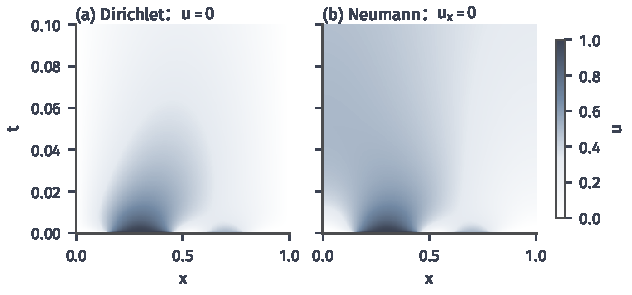
\includegraphics[width=107mm]{figures/03-optimization-evolution-and-signals/02-processes-and-trajectory-evolution/matplotlib/pde-heat-heatmap/figure.pdf}
  \caption{热方程$u_t=u_{xx}$的时空温度图，颜色越深温度越高。初值在$[0.15,0.45]$上为$1$、在$[0.6,0.8]$上为$0.5$，其余为零（边缘做了宽约$0.004$的光滑过渡）。(a)~两端Dirichlet条件$u=0$：温度整体衰减到零。(b)~两端Neumann条件$u_x=0$：温度趋于初值的均值$0.4$。由$400$项正弦与余弦级数计算。}
  \label{fig:pde-heat-heatmap}
\end{figure}

\subsection{弱演化与解算子}
\label{sec:pde-heat-semigroup}

模式展开依赖区间上显式的特征函数。在一般区域上，我们需要不依赖显式公式的框架：一种弱的解释，用能量估计得到唯一性与连续依赖；再把解看成作用在初值上的线性算子族。

\paragraph{弱形式中的时间与空间}
设$\Omega\subset\mathbb R^d$为有界开集，考虑$u_t=\Delta u+f$，边界为零，初值$u_0$。对固定的$t$，用$v\in H_0^1(\Omega)$检验并在空间上分部积分，得到
\begin{equation}
  \frac{\mathrm d}{\mathrm dt}\langle u(t),v\rangle+a\bigl(u(t),v\bigr)=\langle f(t),v\rangle\qquad\text{对所有}v\in H_0^1(\Omega),
  \label{eq:pde-heat-weak}
\end{equation}
其中$a(u,v)=\int_\Omega\nabla u\cdot\nabla v$与上一节相同。要让这个式子有意义，需要分别规定空间与时间上的正则性。在空间上，每个时刻的$u(t)$属于$H_0^1(\Omega)$，即零边界条件与一个弱导数；在时间上，$u$对$t$平方可积地取值于$H_0^1(\Omega)$，而$u_t$只要求取值于$H^{-1}(\Omega)$，这正好与$a(u(t),\cdot)$同属一个空间。初值$u_0$只需属于$L^2(\Omega)$。可以证明满足这些条件的$u$作为$[0,T]\to L^2(\Omega)$的映射是连续的，所以“$u(0)=u_0$”有意义。取值于函数空间的函数的积分（Bochner积分）这里不展开；下面凡需严格论证之处，都落在有限维的Galerkin逼近或区间上的模式展开中完成。

\paragraph{能量估计：唯一性与连续依赖}
在式~\eqref{eq:pde-heat-weak}中取$v=u(t)$。对上述函数类，可以证明$\langle u_t,u\rangle=\tfrac12\tfrac{\mathrm d}{\mathrm dt}\|u\|^2$，于是
\begin{equation}
  \frac12\frac{\mathrm d}{\mathrm dt}\|u(t)\|^2+\|\nabla u(t)\|^2=\langle f(t),u(t)\rangle .
  \label{eq:pde-heat-energy}
\end{equation}
无源时积分得
\[
  \frac12\|u(T)\|^2+\int_0^T\|\nabla u(t)\|^2\,\mathrm dt=\frac12\|u_0\|^2 .
\]
这个等式有两层含义。第一，$\|u(t)\|$不增：两个弱解之差是初值为零的弱解，它的范数恒为零，所以弱解唯一。第二，即使$u_0$只是平方可积、梯度可能处处不存在，梯度的平方在时间上的积分也被$\tfrac12\|u_0\|^2$控制，这是磨光效应的定量形式。有源时，用$|\langle f,u\rangle|\leq\|f\|_{H^{-1}}\|\nabla u\|\leq\tfrac12\|f\|_{H^{-1}}^2+\tfrac12\|\nabla u\|^2$吸收右端，得
\begin{equation}
  \|u(T)\|^2+\int_0^T\|\nabla u\|^2\,\mathrm dt\leq\|u_0\|^2+\int_0^T\|f(t)\|_{H^{-1}}^2\,\mathrm dt .
  \label{eq:pde-heat-energy-source}
\end{equation}
用于两组数据之差，就是初值与源项的连续依赖。

\paragraph{Galerkin逼近构造解}
唯一性与连续依赖来自能量估计，存在性则可以用有限维问题逼近得到。证明思路分三步。

第一步，选$H_0^1(\Omega)$中线性无关的$w_1,w_2,\ldots$，其有限线性组合在$H_0^1(\Omega)$中稠密，例如Dirichlet问题的特征函数。在$V_m=\operatorname{span}\{w_1,\ldots,w_m\}$中找$u_m(t)=\sum_{j=1}^mc_j(t)w_j$，只要求式~\eqref{eq:pde-heat-weak}对$v=w_1,\ldots,w_m$成立。记$\bm M_{i,j}=\langle w_j,w_i\rangle$、$\bm K_{i,j}=a(w_j,w_i)$、$\bm F_i(t)=\langle f(t),w_i\rangle$，条件化为
\[
  \bm M\bm c'(t)+\bm K\bm c(t)=\bm F(t),\qquad\bm c(0)\ \text{由}\ u_0\ \text{在}\ V_m\ \text{上的投影给出}.
\]
$\bm M$是Gram矩阵，对称正定，所以这是常系数线性常微分方程组，由第~\ref{chap:ordinary-differential-equations}章的线性理论在$[0,T]$上有唯一解。

第二步，在有限维中，能量估计~\eqref{eq:pde-heat-energy-source}可以严格推出：$\tfrac12\tfrac{\mathrm d}{\mathrm dt}\bm c^{\top}\bm M\bm c=\bm c^{\top}\bm M\bm c'$只是有限维求导。估计的右端与$m$无关，所以$(u_m)$在相应的函数空间中一致有界。第三步，Hilbert空间中的有界序列有弱收敛子列（这一结论在第~\ref{sec:pde-lax-milgram}小节引用过的卷二同一章中建立）；方程对$u_m$是线性的，对固定的检验函数可以在弱极限下取极限，极限就是弱解。这一构造与第~\ref{sec:pde-fem}小节的有限元方法同源：有限元正是取一组具体的$w_j$，并在有限的$m$处停下来计算。

\paragraph{解算子与半群性质}
固定$f=0$，把初值映到时刻$t$的解，得到映射$S(t):u_0\mapsto u(t)$。由唯一性与线性，$S(t)$是$L^2(\Omega)$上的线性算子；由能量估计，$\|S(t)u_0\|\leq\|u_0\|$。$S(0)$是恒等映射。从$u_0$出发走$t+s$的时间，与先走$s$到达$S(s)u_0$、再以它为初值走$t$，得到同一个解，因为二者在后一段时间满足同一个问题而解唯一，即$S(t+s)=S(t)S(s)$。最后$S(t)u_0\to u_0$，这是初值在$L^2$意义下取到。

上一章的线性系统$\dot{\bm x}=\bm A\bm x$有完全相同的结构：$e^{t\bm A}$满足$e^{0\bm A}=\bm I$与$e^{(t+s)\bm A}=e^{t\bm A}e^{s\bm A}$。热方程的解算子是这一结构在无限维中的对应物，在区间上它把每个$e_k$乘以$e^{-k^2\pi^2t}$，是一个“对角”的指数。

\begin{definition}[强连续半群]
\label{def:pde-c0-semigroup}
设$X$为Banach空间，$\{S(t)\}_{t\geq0}$是$X$上的有界线性算子族。若$S(0)=I$，$S(t+s)=S(t)S(s)$对所有$t,s\geq0$成立，并且对每个$x\in X$，$\lim_{t\to0^+}\|S(t)x-x\|=0$，则称它是\term{强连续半群}（strongly continuous semigroup）。若还有$\|S(t)\|\leq1$，称为压缩半群。
\end{definition}

“半群”指只有$t\geq0$：一般不能把时间倒过来，第~\ref{sec:pde-heat-long-time}小节会看到反向的热方程在何种程度上失效。“强连续”只要求对每个固定的$x$连续，不要求$\|S(t)-I\|\to0$；后者对热方程不成立，因为$\|S(t)e_k-e_k\|=1-e^{-k^2\pi^2t}$在$k\to\infty$时趋于$1$，无论$t$多小。

\paragraph{生成元与定义域}
矩阵指数由$\bm A$生成：$\bm A=\lim_{t\to0}(e^{t\bm A}-\bm I)/t$。对半群做同样的事。

\begin{definition}[生成元]
\label{def:pde-generator}
设$\{S(t)\}$为Banach空间$X$上的强连续半群。令$D(A)$为使极限$\lim_{t\to0^+}(S(t)x-x)/t$在$X$中存在的$x$全体，对$x\in D(A)$令$Ax$为该极限。称$A$为半群的\term{生成元}（generator），$D(A)$为它的定义域。
\end{definition}

区间上的热半群可以把生成元完全算出来。

\begin{theorem}[区间上热半群的生成元]
\label{thm:pde-heat-generator}
在$X=L^2(0,1)$上，设$S(t)$为式~\eqref{eq:pde-heat-series}给出的半群，$\lambda_k=k^2\pi^2$。则$u=\sum_kc_ke_k$属于$D(A)$当且仅当$\sum_k\lambda_k^2c_k^2<\infty$，此时$Au=-\sum_k\lambda_kc_ke_k$。若$u\in H^2(0,1)\cap H_0^1(0,1)$，则$u\in D(A)$且$Au=u''$。
\end{theorem}

\begin{proof}
设$\sum\lambda_k^2c_k^2<\infty$，令$y=-\sum\lambda_kc_ke_k$。则
\[
  \Bigl\|\frac{S(t)u-u}{t}-y\Bigr\|^2=\sum_k\Bigl(\frac{e^{-\lambda_kt}-1}{t}+\lambda_k\Bigr)^2c_k^2 .
\]
由$0\leq1-e^{-\lambda t}\leq\lambda t$，括号中的量属于$[0,\lambda_k]$，每一项不超过$\lambda_k^2c_k^2$，且对每个$k$在$t\to0^+$时趋于零；由控制收敛定理，和趋于零。反过来，若极限$y$存在，取第$k$个系数，$\langle y,e_k\rangle=\lim_{t\to0^+}\frac{e^{-\lambda_kt}-1}{t}c_k=-\lambda_kc_k$，由Parseval等式$\sum\lambda_k^2c_k^2=\|y\|^2<\infty$。

若$u\in H^2\cap H_0^1$，$u$与$e_k$在两端都为零，分部积分两次得$\langle u'',e_k\rangle=\langle u,e_k''\rangle=-\lambda_kc_k$，所以$\sum\lambda_k^2c_k^2=\|u''\|^2<\infty$，且$Au=\sum\langle u'',e_k\rangle e_k=u''$。
\end{proof}

这个计算显示了与矩阵情形的根本差别。$\|Ae_k\|=k^2\pi^2$无界，生成元不是有界算子，只在足够光滑、满足边界条件的函数上有定义；$e^{tA}$不能用幂级数$\sum t^nA^n/n!$定义，只能通过半群本身来理解。边界条件藏在定义域里：Neumann条件给出同一个微分表达式$u''$，但定义域不同，生成的半群也不同。

\paragraph{含源项：Duhamel公式与温和解}
有源项时，回想上一章的常数变易公式：$\dot{\bm x}=\bm A\bm x+\bm f(t)$的解是$\bm x(t)=e^{t\bm A}\bm x_0+\int_0^te^{(t-s)\bm A}\bm f(s)\,\mathrm ds$。区间上逐个模式做同样的计算：第$k$个系数满足标量方程$c_k'=-\lambda_kc_k+f_k(t)$，$f_k=\langle f,e_k\rangle$，所以
\[
  c_k(t)=e^{-\lambda_kt}c_k(0)+\int_0^te^{-\lambda_k(t-s)}f_k(s)\,\mathrm ds .
\]
把所有模式组装起来，就是
\begin{equation}
  u(t)=S(t)u_0+\int_0^tS(t-s)f(s)\,\mathrm ds ,
  \label{eq:pde-duhamel}
\end{equation}
称为\term{Duhamel公式}（Duhamel's formula）。右端可以这样读：时刻$s$注入的热量$f(s)\,\mathrm ds$此后自由扩散了$t-s$的时间，再与初值的扩散叠加。

设$f:[0,T]\to L^2(\Omega)$连续。半群一致有界且强连续，所以被积函数$s\mapsto S(t-s)f(s)$连续，式~\eqref{eq:pde-duhamel}可以作为取值于$L^2$的连续函数的Riemann积分理解。我们把由式~\eqref{eq:pde-duhamel}定义的$u$称为温和解。它不要求$u$可微，只要求半群存在，因而适用于数据较粗糙的情形；数据足够好时，可以证明它与弱解、经典解一致。

\begin{example}[恒定热源下趋于稳态]
\label{ex:pde-heat-steady-source}
在$(0,1)$上取$u_0=0$、恒定热源$f=1$、两端为零。$f$的系数为$f_k=\langle1,e_k\rangle$，由Duhamel公式$c_k(t)=f_k(1-e^{-\lambda_kt})/\lambda_k$。$t\to\infty$时$c_k(t)\to f_k/\lambda_k$，这正是稳态问题$-u''=1$的解$x(1-x)/2$的系数，因为$-u''=f$在模式坐标中就是$\lambda_kc_k=f_k$。每个模式以自己的速率$\lambda_k$接近稳态，最慢的是$k=1$。
\end{example}

\paragraph{一般区域上的生成元（补充）}
在一般有界区域上没有显式的特征函数，生成元要直接构造。令$D(A)$由满足下述条件的$u\in H_0^1(\Omega)$组成：存在$g\in L^2(\Omega)$，使$a(u,v)=-\langle g,v\rangle$对所有$v\in H_0^1(\Omega)$成立；对这样的$u$令$Au=g$，它是弱意义下的$\Delta u$。这个算子有两条性质。其一，$\langle Au,u\rangle=-\|\nabla u\|^2\leq0$，称为耗散的。其二，对每个$\lambda>0$与$f\in L^2(\Omega)$，方程$\lambda u-Au=f$可解，因为它的弱形式$\lambda\langle u,v\rangle+a(u,v)=\langle f,v\rangle$的双线性型在$H_0^1$上强制，可以用Lax--Milgram定理。泛函分析中的Lumer--Phillips定理说，稠密定义、耗散且$\lambda I-A$满射的算子恰好生成压缩半群；这里不加证明地引用它。于是热半群在一般区域上同样存在，前面的能量估计、半群性质和Duhamel公式都照样成立。

\subsection{能量、正性与长期极限}
\label{sec:pde-heat-long-time}

\paragraph{能量耗散、总热量守恒与边界泄漏}
本小节设解足够光滑，可以在空间上分部积分。考察两个量：能量$E(t)=\tfrac12\|u(t)\|^2$与总热量$Q(t)=\int_\Omega u(\bm x,t)\,\mathrm d\bm x$。无源时，
\[
  \begin{aligned}
    E'(t)&=\int_\Omega u\Delta u\,\mathrm d\bm x=-\|\nabla u\|^2+\int_{\partial\Omega}u\,\partial_{\bm n}u\,\mathrm dS,\\
    Q'(t)&=\int_\Omega\Delta u\,\mathrm d\bm x=\int_{\partial\Omega}\partial_{\bm n}u\,\mathrm dS .
  \end{aligned}
\]
零Dirichlet与零Neumann边界都使$E'$的边界项为零，所以$E'=-\|\nabla u\|^2\leq0$，能量耗散。总热量则不同：零Neumann边界下$Q'=0$，热量守恒；零Dirichlet边界下$Q'$等于穿过边界的净通量，正温度场在边界附近向零下降，$\partial_{\bm n}u\leq0$，热量从边界泄漏。

所以“能量耗散”“总量守恒”“边界泄漏”是三个不同的性质，不能互相推出。绝热的棒保持总热量，能量仍在减少：由Cauchy--Schwarz不等式$Q^2\leq|\Omega|\,\|u\|^2$，在总热量固定时，均匀分布的温度能量最小，扩散让温度趋于均匀，能量随之下降到这个最小值。图~\ref{fig:pde-heat-energy-max}(a)在两端为零的情形下比较了能量与总热量：二者都衰减，但速率不同。

\paragraph{弱最大值原理}
热量从热处流向冷处，所以内部不可能凭空出现比初始和边界更热的点。下面的定理把这一直觉变成证明，这类结论统称\term{最大值原理}（maximum principle）。记$\Omega_T=\Omega\times(0,T]$，称$\Gamma_T=(\overline\Omega\times\{0\})\cup(\partial\Omega\times[0,T])$为抛物边界，即底面与侧面，不含顶面。

\begin{theorem}[热方程的弱最大值原理]
\label{thm:pde-max-principle}
设$\Omega$为有界开集，$\kappa>0$，$u$在$\Omega_T$上关于$\bm x$二次、关于$t$一次连续可微，并在$\overline\Omega\times[0,T]$上连续。若在$\Omega_T$中$u_t-\kappa\Delta u\leq0$，则
\[
  \max_{\overline\Omega\times[0,T]}u=\max_{\Gamma_T}u .
\]
\end{theorem}

\begin{proof}
任取$\varepsilon>0$，令$v=u-\varepsilon t$，则在$\Omega_T$中$v_t-\kappa\Delta v=u_t-\kappa\Delta u-\varepsilon<0$。$v$在紧集$\overline\Omega\times[0,T]$上连续，在某点$(\bm x_0,t_0)$取到最大值。假设该点在$\Omega_T$中，即$\bm x_0\in\Omega$、$0<t_0\leq T$。固定$t_0$，$\bm x_0$是$v(\cdot,t_0)$的内部最大点，Hessian半负定，$\Delta v\leq0$。固定$\bm x_0$，若$t_0<T$则$v_t=0$；若$t_0=T$，$v(\bm x_0,t)\leq v(\bm x_0,T)$对$t<T$成立，左导数$v_t\geq0$。两种情形都有$v_t-\kappa\Delta v\geq0$，矛盾。所以最大值在$\Gamma_T$上取到，
\[
  \max u\leq\max v+\varepsilon T=\max_{\Gamma_T}v+\varepsilon T\leq\max_{\Gamma_T}u+\varepsilon T .
\]
令$\varepsilon\to0$即得。
\end{proof}

对$-u$使用定理，最小值也在抛物边界上取到。由此得到几个直接的推论。\term{比较原理}（comparison principle）：若$u_t-\kappa\Delta u\leq w_t-\kappa\Delta w$且在$\Gamma_T$上$u\leq w$，则处处$u\leq w$，只需对$u-w$使用定理。正性：无源时，初值与边界值非负，则解处处非负。稳定性与唯一性：两个经典解之差满足$\max|u_1-u_2|\leq\max_{\Gamma_T}|u_1-u_2|$，数据相同则解相同。图~\ref{fig:pde-heat-energy-max}(b)画出了初值$\sin(\pi x)+\sin(5\pi x)$的最大值$M(t)$与最小值$m(t)$：前者单调不增，后者从$-0.198$单调回升到零，从未越出初值的范围。定理~\ref{thm:pde-max-principle}在上述的弱形式中也有相应版本，这里只讨论经典解。

\begin{figure}[!htb]
  \centering
  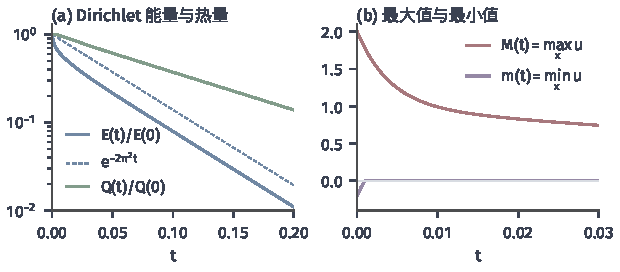
\includegraphics[width=105mm]{figures/03-optimization-evolution-and-signals/02-processes-and-trajectory-evolution/matplotlib/pde-heat-energy-max/figure.pdf}
  \caption{两端为零的热方程$u_t=u_{xx}$中的能量、热量与极值。(a)~初值与图~\ref{fig:pde-heat-heatmap}相同，能量$E=\tfrac12\|u\|^2$与总热量$Q=\int u$都相对初值归一化，纵轴为对数刻度；虚线$e^{-2\pi^2t}$是由Poincaré不等式得到的能量上界。(b)~初值$\sin(\pi x)+\sin(5\pi x)$的空间最大值$M(t)$与最小值$m(t)$，二者都不越出初值和边界值的范围。}
  \label{fig:pde-heat-energy-max}
\end{figure}

\paragraph{长期行为：衰减、均值与稳态}
在零Dirichlet边界下，由Poincaré不等式$\|\nabla u\|^2\geq\|u\|^2/C_P^2$，能量满足$E'\leq-2E/C_P^2$，于是$\frac{\mathrm d}{\mathrm dt}\bigl(e^{2t/C_P^2}E\bigr)\leq0$，
\[
  \|u(t)\|\leq e^{-t/C_P^2}\|u_0\| .
\]
在$(0,1)$上$C_P=1/\pi$，速率$\pi^2$正是最低模式的衰减率，与定理~\ref{thm:pde-heat-series}一致；图~\ref{fig:pde-heat-energy-max}(a)的虚线就是这个界。

在零Neumann边界下，总热量守恒，均值$\bar u=Q/|\Omega|$不随时间变化。$w=u-\bar u$满足同一方程、同一边界条件，且均值为零；设$\Omega$为有界连通Lipschitz区域，由零均值的Poincaré不等式，同样的论证给出$\|u(t)-\bar u\|\leq e^{-t/C^2}\|u_0-\bar u\|$。解趋于初值的均值，不趋于零，这就是图~\ref{fig:pde-heat-heatmap}(b)中的现象。

有不随时间变化的源$f\in L^2(\Omega)$时，零Dirichlet边界下令$u_\infty$为Poisson问题$-\Delta u_\infty=f$的弱解。$w=u-u_\infty$满足无源的热方程，初值为$u_0-u_\infty$，所以$\|u(t)-u_\infty\|\leq e^{-t/C_P^2}\|u_0-u_\infty\|$：有源时解趋于稳态，而不是趋于零，例~\ref{ex:pde-heat-steady-source}是它的具体情形。零Neumann边界下，若$\int_\Omega f\neq0$，则$Q'=\int_\Omega f$，总热量线性增长，没有稳态；这正是第~\ref{sec:pde-other-boundary}小节的相容条件在时间中的表现，图~\ref{fig:pde-neumann}(b)画出了这种情形。

\paragraph{反向热方程不适定}
磨光效应的另一面是信息的丢失。设已知时刻$T$的温度，反推初值。在区间上，$c_k(0)=e^{k^2\pi^2T}c_k(T)$。若时刻$T$的观测有一个大小为$\delta$的高频误差$\delta e_k$，反推出的初值误差就是$\delta e^{k^2\pi^2T}e_k$。取$T=0.1$、$k=5$，放大倍数$e^{2.5\pi^2}\approx5\times10^{10}$；$k$越大放大越厉害，没有上界。所以反向问题在$L^2$中不满足连续依赖，按第~\ref{sec:pde-boundary-solution-meaning}小节的定义是不适定的。正向演化把高频成分压到几乎为零，反向演化就必须把几乎为零的成分重新放大。

本节始终把$u$当作确定性的温度场。热方程还有一个概率的读法：它也描述随机游走的粒子在空间中的密度怎样随时间扩散。这一联系需要随机过程的生成元，留到第~\ref{chap:continuous-time-stochastic-processes}章建立。

% 第3章第4节：输运方程与传播（特征线与初值解；守恒形式与间断）。

\section{输运方程与传播}
\label{sec:pde-transport}

扩散把场抹平，输运则把场搬走。本节研究给定速度场怎样搬运一个初始场。关键的想法是跟着流动走：沿着速度场的轨迹，偏微分方程变成上一章的常微分方程。我们还要区分两种搬运：搬运的是场的数值（如染料的颜色），还是场所代表的质量（如染料的浓度）；最后看到，当速度依赖场本身时，轨迹会相撞，光滑的解会在有限时间内破裂。

\subsection{特征线与初值解}
\label{sec:pde-characteristics}

\paragraph{常速度平移}
想象一条以恒定速度$b$流动的河，水中溶有一种示踪物，$u(x,t)$是它在位置$x$、时刻$t$的颜色深浅。示踪物不扩散，只随水流走，于是\term{输运方程}（transport equation）
\begin{equation}
  u_t+bu_x=0,\qquad u(x,0)=u_0(x)
  \label{eq:pde-transport-constant}
\end{equation}
描述它的变化。站在岸上看，某处的颜色在变；坐在随水漂流的小船上看，周围的颜色不变。设小船位置为$X(t)=y+bt$，由链式法则
\[
  \frac{\mathrm d}{\mathrm dt}u(X(t),t)=u_x(X(t),t)\,X'(t)+u_t(X(t),t)=bu_x+u_t=0,
\]
所以$u$沿着这条线保持初值$u_0(y)$。给定$(x,t)$，反解出出发点$y=x-bt$，得$u(x,t)=u_0(x-bt)$。若$u_0\in C^1(\mathbb R)$，直接求导可验证它是经典解；上面的推导同时说明任何$C^1$解都必须是它，所以解唯一。

在$(x,t)$平面中，直线$x-bt=y$称为\term{特征线}（characteristic）。图~\ref{fig:pde-characteristics}(a)画出了这些平行直线，颜色是解的值：鼓包沿特征线原封不动地平移。

\begin{figure}[!htb]
  \centering
  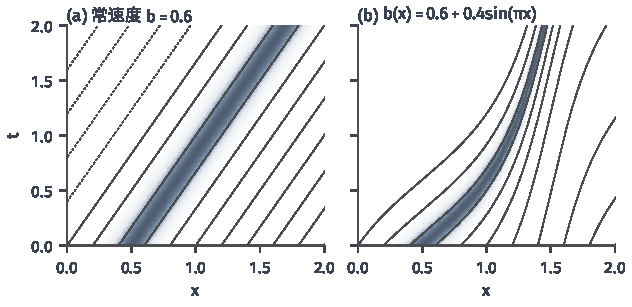
\includegraphics[width=107mm]{figures/03-optimization-evolution-and-signals/02-processes-and-trajectory-evolution/matplotlib/pde-characteristics/figure.pdf}
  \caption{输运方程$u_t+b(x)u_x=0$在$[0,2]$上的特征线（细线）与解（颜色越深值越大），初值$u_0=\exp(-((x-0.5)/0.15)^2)$，左端流入边界上给定$u(0,t)=0$。(a)~常速度$b=0.6$：特征线是平行直线，实线从$t=0$出发，虚线从流入边界出发。(b)~$b(x)=0.6+0.4\sin(\pi x)$：特征线在速度快处变陡，在$x=1.5$附近速度最慢处聚拢，鼓包沿途保持高度、宽度被压缩。特征线由四阶Runge--Kutta法积分。}
  \label{fig:pde-characteristics}
\end{figure}

\paragraph{变速度场与特征线方程}
速度随位置和时间变化时，小船的轨迹不再是直线，但道理相同。在$\mathbb R^d$中考虑
\begin{equation}
  u_t+\bm b(\bm x,t)\cdot\nabla u=0,\qquad u(\bm x,0)=u_0(\bm x).
  \label{eq:pde-transport}
\end{equation}
沿着曲线$\bm X(t)$，$\frac{\mathrm d}{\mathrm dt}u(\bm X(t),t)=\nabla u\cdot\bm X'+u_t$，它为零的条件正是$\bm X'=\bm b(\bm X,t)$。所以特征线就是速度场的轨线：
\begin{equation}
  \dot{\bm X}(t)=\bm b(\bm X(t),t),\qquad\bm X(0)=\bm y .
  \label{eq:pde-characteristic-ode}
\end{equation}
这是第~\ref{chap:ordinary-differential-equations}章的初值问题。若$\bm b$连续、关于$\bm x$连续可微且$D_{\bm x}\bm b$有界，则它关于$\bm x$整体Lipschitz，对每个$\bm y$有定义在全部$t\geq0$上的唯一解。记$\Phi_t(\bm y)=\bm X(t)$为时刻$t$的流映射。由唯一性，从时刻$t$的点$\bm x$反向求解式~\eqref{eq:pde-characteristic-ode}得到唯一的出发点，所以$\Phi_t$是$\mathbb R^d$上的双射；并且$\bm b$关于$\bm x$连续可微时，流映射及其逆关于初值连续可微，这是可微依赖定理的结论，这里引用而不证明。

\begin{theorem}[输运方程的特征线解]
\label{thm:pde-transport-characteristics}
设$\bm b$满足上述条件，$u_0\in C^1(\mathbb R^d)$。则$u(\bm x,t)=u_0\bigl(\Phi_t^{-1}(\bm x)\bigr)$是式~\eqref{eq:pde-transport}的唯一$C^1$解。
\end{theorem}

\begin{proof}
唯一性：若$u$是$C^1$解，上面的链式法则说明$u(\Phi_t(\bm y),t)$关于$t$的导数为零，所以$u(\Phi_t(\bm y),t)=u_0(\bm y)$；每个$(\bm x,t)$都在唯一一条特征线上，取$\bm y=\Phi_t^{-1}(\bm x)$即得公式。存在性：公式定义的$u$是$C^1$函数的复合，连续可微；沿每条特征线它等于常数$u_0(\bm y)$，对$t$求导即得在点$(\Phi_t(\bm y),t)$处$u_t+\bm b\cdot\nabla u=0$，而这些点覆盖了整个$\mathbb R^d\times[0,\infty)$。
\end{proof}

解的值沿特征线不变，但形状可以变。一维时取$b(x)=x$，特征线$X=ye^t$，解$u=u_0(xe^{-t})$：初值被横向拉伸$e^t$倍，高度不变。图~\ref{fig:pde-characteristics}(b)中速度先快后慢，鼓包进入慢速区时前端先减速、后端追上来，于是被压窄。

\paragraph{源项沿特征线累计}
若示踪物在流动中还被注入或分解，方程变为$u_t+\bm b\cdot\nabla u=s(\bm x,t)$。沿特征线，$\frac{\mathrm d}{\mathrm dt}u(\bm X(t),t)=s(\bm X(t),t)$，积分得
\[
  u\bigl(\Phi_t(\bm y),t\bigr)=u_0(\bm y)+\int_0^ts\bigl(\Phi_\tau(\bm y),\tau\bigr)\,\mathrm d\tau .
\]
例如$b=1$、$s=1$时$u=u_0(x-t)+t$：小船上的人看到颜色每单位时间加深$1$。若还有按比例的分解$-cu$，沿特征线就得到线性常微分方程$U'=-cU+s$，用常数变易法求解。输运方程于是化为一族以出发点$\bm y$为参数的常微分方程，每条特征线各自独立地计算。

\paragraph{有界区域：只在流入边界给数据}
在区间$(0,1)$上取$b=1$。特征线从左端流入，从右端流出。初值$u_0$只决定从底边出发的特征线上的值；从左端$x=0$进入的特征线还需要另外的数据，所以给定$u(0,t)=g(t)$，解为
\[
  u(x,t)=\begin{cases}u_0(x-t),&x\geq t,\\ g(t-x),&x<t .\end{cases}
\]
右端$x=1$处的值已经被沿特征线搬来的数据决定，再规定它会与之冲突。一般地，边界上只能在\term{流入边界}（inflow boundary）$\{\bm x\in\partial\Omega:\bm b\cdot\bm n<0\}$给数据，这与热方程在整个边界上给数据完全不同。若$u_0(0)\neq g(0)$，解在特征线$x=t$上有一个跳跃，它被原样搬向下游，永不磨光，这与第~\ref{sec:pde-boundary-solution-meaning}小节关于相容条件的讨论相呼应。图~\ref{fig:pde-characteristics}中的虚线就是从流入边界出发的特征线，那里的值来自$g=0$。

\paragraph{反向追踪的条件}
公式$u_0(\Phi_t^{-1}(\bm x))$依赖于每个点恰好有一条特征线经过。速度场不够正则时，这一点可以失败。取$b(x)=2\sqrt{|x|}$，它连续但在原点不满足Lipschitz条件。从原点出发，$X\equiv0$与$X=t^2$都是$X'=2\sqrt{|X|}$的解；还可以在原点停留任意时间$\tau$后再出发，$X=(t-\tau)^2$。从$x>0$、$t>\sqrt x$的点反向追踪，可以回到$y=0$，也可以经过原点后回到任何$y\in[-(t-\sqrt x)^2,0]$。于是$u(x,t)$等于$u_0$在这些点中哪一处的值无法确定，输运方程有多个解。特征线方法的使用条件就是流映射存在、唯一，并且特征线覆盖了需要求解的区域。

\subsection{守恒形式与间断}
\label{sec:pde-conservation}

\paragraph{搬运数值与搬运质量}
前面的$u$是一种“标签”：颜色深浅随水移动，但不关心水被压缩还是拉伸。若要描述的是单位体积中的质量，即密度$\rho$，压缩的水流会让密度升高。用第~\ref{sec:pde-heat-modes}小节同样的守恒推理，区域内质量的变化等于穿过边界的通量$\rho\bm b$，得到\term{连续性方程}（continuity equation）
\begin{equation}
  \rho_t+\nabla\cdot(\bm b\rho)=0 .
  \label{eq:pde-continuity}
\end{equation}
展开散度，$\nabla\cdot(\bm b\rho)=\bm b\cdot\nabla\rho+\rho\nabla\cdot\bm b$，所以沿特征线
\[
  \frac{\mathrm d}{\mathrm dt}\rho\bigl(\bm X(t),t\bigr)=-\rho\,\nabla\cdot\bm b .
\]
与式~\eqref{eq:pde-transport}对比，差别只在散度一项：流动压缩（$\nabla\cdot\bm b<0$）处密度沿途增加，流动扩张处密度减少；速度场无散度时两个方程相同。式~\eqref{eq:pde-continuity}的通量写在散度号里，称为\term{守恒形式}（conservative form）。

数值不变与质量不变是两个不同的守恒性质。设$A$为一块初始区域，$\Phi_t(A)$是它随流运动到时刻$t$的位置，下面证明$\int_{\Phi_t(A)}\rho\,\mathrm d\bm x$不随时间变化。令$J_t(\bm y)=\det D\Phi_t(\bm y)$。$D\Phi_t$满足变分方程$\frac{\mathrm d}{\mathrm dt}D\Phi_t=D_{\bm x}\bm b(\Phi_t,t)\,D\Phi_t$，由行列式求导公式$\frac{\mathrm d}{\mathrm dt}\det\bm M=\det\bm M\operatorname{tr}(\bm M^{-1}\bm M')$，得$\frac{\mathrm d}{\mathrm dt}J_t=(\nabla\cdot\bm b)(\Phi_t,t)\,J_t$，且$J_0=1$，所以$J_t>0$。换元得
\[
  \int_{\Phi_t(A)}\rho(\bm x,t)\,\mathrm d\bm x=\int_A\rho\bigl(\Phi_t(\bm y),t\bigr)J_t(\bm y)\,\mathrm d\bm y,
\]
被积函数对$t$的导数是$J_t\bigl(\frac{\mathrm d}{\mathrm dt}\rho+\rho\nabla\cdot\bm b\bigr)=0$。体积被压缩多少，密度就升高多少，二者乘积不变。

\begin{example}[收缩流中的数值与密度]
\label{ex:pde-compressing-flow}
取一维速度$b(x)=-x$，流体向原点收缩，特征线$X=ye^{-t}$。数值方程$u_t-xu_x=0$的解为$u=u_0(xe^t)$：形状横向压缩$e^t$倍，高度不变。连续性方程$\rho_t-(x\rho)_x=0$中$\nabla\cdot b=-1$，沿特征线$\frac{\mathrm d}{\mathrm dt}\rho=\rho$，所以$\rho(x,t)=e^t\rho_0(xe^t)$：形状同样被压缩，高度却升高$e^t$倍，总质量$\int\rho\,\mathrm dx=\int\rho_0\,\mathrm dx$不变。
\end{example}

图~\ref{fig:pde-transport-vs-continuity}把这两种搬运并排画出。若把一个随机初始状态放进常微分方程演化，它的概率密度满足的正是连续性方程；第~\ref{chap:continuous-time-stochastic-processes}章在加入随机扰动后会得到相应的密度方程。

\begin{figure}[!htb]
  \centering
  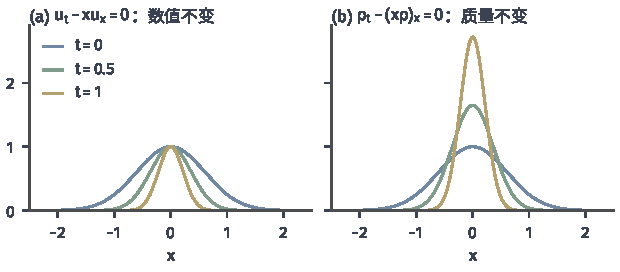
\includegraphics[width=105mm]{figures/03-optimization-evolution-and-signals/02-processes-and-trajectory-evolution/matplotlib/pde-transport-vs-continuity/figure.pdf}
  \caption{收缩速度场$b(x)=-x$下的两种搬运（例~\ref{ex:pde-compressing-flow}），初值同为$\exp(-x^2/0.72)$，三种颜色依次为$t=0,0.5,1$。(a)~输运方程：数值沿特征线不变，峰高保持$1$。(b)~连续性方程：峰高依次为$1$、$e^{0.5}\approx1.65$、$e\approx2.72$，曲线下面积保持约$1.504$。}
  \label{fig:pde-transport-vs-continuity}
\end{figure}

\paragraph{积分形式的守恒律}
在一维中，许多守恒量满足形如
\begin{equation}
  u_t+\bigl(F(u)\bigr)_x=0
  \label{eq:pde-conservation-law}
\end{equation}
的方程，称为\term{守恒律}（conservation law），$F$是通量函数。线性输运对应$F(u)=bu$；交通流中$u$是车辆密度，$F(u)=u\,v(u)$，车速$v$随密度增大而降低。式~\eqref{eq:pde-conservation-law}来自积分形式
\[
  \frac{\mathrm d}{\mathrm dt}\int_a^bu\,\mathrm dx=F\bigl(u(a,t)\bigr)-F\bigl(u(b,t)\bigr),
\]
即区间内的总量变化等于左端流入减右端流出。积分形式只要求$u$可积，对有跳跃的$u$也有意义；微分形式需要$u$可微。下面会看到，这个区别在非线性情形中不可回避。

\paragraph{Burgers方程中的特征线交叉}
取$F(u)=u^2/2$，对光滑的$u$，式~\eqref{eq:pde-conservation-law}即\allowbreak\term{Burgers方程}（Burgers' equation）$u_t+uu_x=0$。它与输运方程的区别是：速度不再是给定的$b$，而是$u$本身。沿用小船的论证，特征线满足$X'=u(X,t)$，而$u$沿特征线不变，所以特征线仍是直线
\[
  X(t)=y+u_0(y)\,t,
\]
只是不同出发点的直线斜率不同：值大的点跑得快。若$u_0$在某处递减，后面跑得快的点就会追上前面跑得慢的点。

固定$t$，映射$y\mapsto y+u_0(y)t$的导数是$1+u_0'(y)t$。只要它保持为正，特征线不相交，$u$由$u_0$经此映射的逆唯一确定，并且由$u(X(t),t)=u_0(y)$对$y$求导得$u_x=u_0'(y)/(1+u_0'(y)t)$。若$u_0'$在某处为负，最早在
\[
  t_*=\frac1{\max_y\bigl(-u_0'(y)\bigr)}
\]
时刻，导数$1+u_0'(y)t$在使$-u_0'$最大的点处变为零，$u_x$趋于$-\infty$：初值再光滑，经典解也在有限时间内失效。取$u_0=e^{-x^2}$，$-u_0'=2xe^{-x^2}$在$y=1/\sqrt2$处取最大值$\sqrt2e^{-1/2}\approx0.858$，所以$t_*\approx1.166$，交叉发生在$x=y+u_0(y)t_*=\sqrt2$。图~\ref{fig:pde-burgers}(a)画出了这些特征线：鼓包后坡的直线在$t_*$处开始交叉。

过了$t_*$，若仍沿特征线搬运数值，同一个$x$会被几条特征线带来不同的值，剖面变成图~\ref{fig:pde-burgers}(b)中虚线那样的S形，不再是函数的图像。物理上，前方的车辆堆积时不会穿过彼此，而是形成一个密度跳跃。我们需要允许间断的解。

\begin{figure}[!htb]
  \centering
  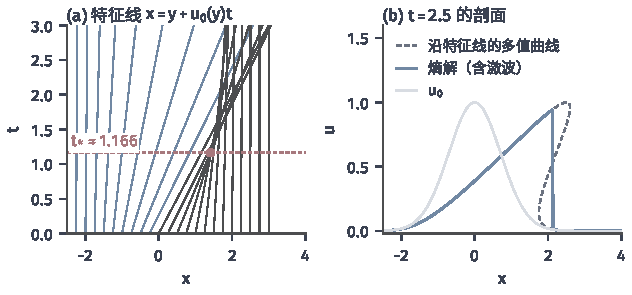
\includegraphics[width=107mm]{figures/03-optimization-evolution-and-signals/02-processes-and-trajectory-evolution/matplotlib/pde-burgers/figure.pdf}
  \caption{Burgers方程$u_t+(u^2/2)_x=0$，初值$u_0=e^{-x^2}$。(a)~特征线$x=y+u_0(y)t$，蓝色从$y<0$出发、深灰色从$y\geq0$出发；圆点为最早的交叉点$(\sqrt2,t_*)$，$t_*\approx1.166$。(b)~$t=2.5$时的剖面：虚线是沿特征线搬运得到的多值曲线；实线是用Godunov有限体积格式（$4000$个网格，CFL数$0.45$）计算的熵解，在$x\approx2.12$处有激波；浅灰线是初值。}
  \label{fig:pde-burgers}
\end{figure}

\paragraph{弱解、Rankine--Hugoniot条件与熵条件}
对光滑解，用$\varphi\in C_c^1(\mathbb R\times[0,\infty))$乘以式~\eqref{eq:pde-conservation-law}并在$x$与$t$上分部积分，得到
\[
  \int_0^\infty\!\!\int_{\mathbb R}\bigl(u\varphi_t+F(u)\varphi_x\bigr)\,\mathrm dx\,\mathrm dt+\int_{\mathbb R}u_0(x)\varphi(x,0)\,\mathrm dx=0 .
\]
导数全部转移到了测试函数上，这个式子对有界可测的$u$也有意义。称对所有这样的$\varphi$满足上式的$u$为守恒律的弱解，这与第~\ref{sec:pde-weak-form}小节的想法相同。

弱解允许跳跃，但跳跃不能随意移动。设解在$x=s(t)$处有一个跳跃，左侧值$u_L$、右侧值$u_R$。在包含$s(t)$的小区间$[a,b]$上用积分形式，区间很短时两侧近似为常数，总量约为$(s-a)u_L+(b-s)u_R$，它对$t$的导数为$s'(u_L-u_R)$，必须等于$F(u_L)-F(u_R)$。于是得到\term{Rankine--Hugoniot条件}（Rankine--Hugoniot condition）
\[
  s'(t)=\frac{F(u_L)-F(u_R)}{u_L-u_R} .
\]
对Burgers方程，$s'=(u_L+u_R)/2$，跳跃以两侧值的平均速度移动。这样移动的跳跃称为\term{激波}（shock wave）。

可是弱解不一定唯一。取初值在$x<0$为$0$、在$x>0$为$1$。一方面，$u_L=0$、$u_R=1$的跳跃以速度$1/2$移动，满足Rankine--Hugoniot条件，是一个弱解。另一方面，令$u=0$（$x<0$），$u=x/t$（$0\leq x\leq t$），$u=1$（$x>t$），直接验证$u_t+uu_x=-x/t^2+(x/t)(1/t)=0$，它连续且是另一个弱解，称为\term{稀疏波}（rarefaction wave）。需要额外的选择规则。对凸的$F$，Lax提出的\term{熵条件}（entropy condition）要求两侧的特征线都流入激波：$F'(u_L)>s'>F'(u_R)$，对Burgers方程即$u_L>s'>u_R$。上例中$u_L=0<u_R=1$，跳跃违反熵条件，物理的解是稀疏波；反过来$u_L=1$、$u_R=0$的跳跃满足熵条件，是真正的激波。

满足熵条件的弱解也可以理解为加一点扩散再取极限：$u_t+uu_x=\varepsilon u_{xx}$在$\varepsilon\to0$时的解趋于熵解，激波是被极小的扩散磨成的一段陡峭过渡。图~\ref{fig:pde-burgers}(b)中的数值格式自带少量数值扩散，算出的正是熵解。非线性守恒律的熵解理论，包括一般通量下的存在唯一性，本章不展开；这里只需看到两点：非线性可以让光滑解在有限时间内产生间断，这时必须扩大解的范围，并补充选择物理解的条件。

% 第3章第5节：波动方程与能量传播（初值解与传播速度；能量估计与解的稳定性）。

\section{波动方程与能量传播}
\label{sec:pde-wave}

热方程中曲率决定变化的速度，波动方程中曲率决定变化的加速度。多出的这一阶时间导数让场具有惯性：它会越过平衡位置，把扰动以有限速度传向远处，并且不会自行停下来。本节先在全直线和区间上求出解，看清传播与反射；再用能量估计证明唯一性和连续依赖，并与热方程的耗散对照。

\subsection{初值解与传播速度}
\label{sec:pde-wave-solution}

\paragraph{弦的振动方程}
设一根弦沿$x$轴绷紧，张力为$T$，线密度为$\rho$，$u(x,t)$是它在$x$处的竖直位移。取一小段$[a,b]$，两端的张力沿弦的切线方向，竖直分量约为$T\sin\theta\approx T\tan\theta=Tu_x$，这里用了小斜率近似。净竖直力为$T\bigl(u_x(b,t)-u_x(a,t)\bigr)=\int_a^bTu_{xx}\,\mathrm dx$。由Newton第二定律，它等于这一段的质量乘加速度$\int_a^b\rho u_{tt}\,\mathrm dx$。区间任意，得到\term{波动方程}（wave equation）
\begin{equation}
  u_{tt}=c^2u_{xx},\qquad c=\sqrt{T/\rho} .
  \label{eq:pde-wave-1d}
\end{equation}
推导忽略了弦的水平运动、重力与空气阻力，并假设斜率很小。在$d$维中，膜的振动与声波满足$u_{tt}=c^2\Delta u$。

方程对时间是二阶的，所以需要两个初值：初位移$u(x,0)=u_0(x)$与初速度$u_t(x,0)=u_1(x)$。这与上一章的二阶常微分方程$\ddot x=-\omega^2x$需要初始位置和速度是同一回事；更准确地说，场的状态是一对函数$(u,u_t)$，而不只是位移。

\paragraph{d'Alembert公式}
在整条实轴上，方程可以完全解出。对$C^2$函数，混合偏导数可交换，于是$u_{tt}-c^2u_{xx}=(\partial_t-c\partial_x)(\partial_t+c\partial_x)u$：波动算子是两个一阶输运算子的乘积，一个向右、一个向左。引入特征坐标$\xi=x-ct$、$\eta=x+ct$，方程变为$u_{\xi\eta}=0$，所以$u_\xi$与$\eta$无关，积分两次得$u=F(\xi)+G(\eta)$：解是一个右行波与一个左行波之和。

用初值确定$F$与$G$：$F+G=u_0$，$-cF'+cG'=u_1$。后者积分得$G-F=c^{-1}\int_0^xu_1+K$，与前者联立解出$F,G$，代回得
\begin{equation}
  u(x,t)=\frac12\bigl[u_0(x-ct)+u_0(x+ct)\bigr]+\frac1{2c}\int_{x-ct}^{x+ct}u_1(s)\,\mathrm ds .
  \label{eq:pde-dalembert}
\end{equation}
这就是\term{d'Alembert公式}（d'Alembert's formula）。若$u_0\in C^2(\mathbb R)$、$u_1\in C^1(\mathbb R)$，可以直接验证它是$C^2$解：$t=0$时第一项为$u_0$、第二项为零；对$t$求导再令$t=0$，第一项给出$\tfrac12[-cu_0'+cu_0']=0$，第二项给出$\tfrac1{2c}[cu_1(x)+cu_1(x)]=u_1(x)$。上面的推导又说明每个$C^2$解都具有这一形式，所以解唯一。

初速度为零时，初始形状分成两半，各以速度$c$向左右跑开，形状不变。图~\ref{fig:pde-dalembert}(a)画出了这一过程：$t=0.75$时两半还有重叠，之后完全分开，各自的高度都是原来的一半。

\begin{figure}[!htb]
  \centering
  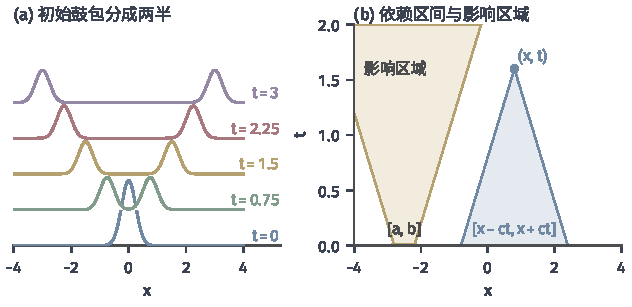
\includegraphics[width=107mm]{figures/03-optimization-evolution-and-signals/02-processes-and-trajectory-evolution/matplotlib/pde-dalembert/figure.pdf}
  \caption{全直线上的波动方程，$c=1$。(a)~初位移$u_0=e^{-(x/0.35)^2}$、初速度为零的d'Alembert解在五个时刻的形状，竖直方向错开排列：鼓包分成两个半高的行波。(b)~$(x,t)$平面中的依赖与影响：点$(x,t)$的值只依赖初始数据在蓝色三角形底边$[x-ct,x+ct]$上的值；支撑在$[a,b]$上的初始数据只影响黄色区域$[a-ct,b+ct]$。}
  \label{fig:pde-dalembert}
\end{figure}

\paragraph{有限传播速度}
式~\eqref{eq:pde-dalembert}显示，点$(x,t)$处的值只依赖$u_0$在两点$x\pm ct$处的值和$u_1$在区间$[x-ct,x+ct]$上的值。这个区间称为点$(x,t)$的\term{依赖区域}（domain of dependence）。反过来，若初始数据在$[a,b]$外为零，那么在时刻$t$，解在$[a-ct,b+ct]$外为零，扰动只影响这个以速度$c$扩张的\term{影响区域}（domain of influence）。图~\ref{fig:pde-dalembert}(b)画出了这两个区域：信号以有限速度$c$传播。

热方程完全不同。在全直线上，可以直接验证热核
\[
  \Phi(x,t)=\frac1{\sqrt{4\pi\kappa t}}\exp\Bigl(-\frac{x^2}{4\kappa t}\Bigr),\qquad t>0
\]
满足$\Phi_t=\kappa\Phi_{xx}$：两边都等于$\Phi\cdot\bigl(-\tfrac1{2t}+\tfrac{x^2}{4\kappa t^2}\bigr)$。对有界连续的初值，$u(x,t)=\int\Phi(x-y,t)u_0(y)\,\mathrm dy$给出热方程的解，图~\ref{fig:pde-three-mechanisms}(a)中Gauss鼓包方差增大$2\kappa t$正是这个卷积的结果。由于$\Phi$处处为正，只要$u_0\geq0$且不恒为零，任意$t>0$时$u(x,t)$在所有$x$处都为正：一点的加热瞬间被无穷远处感知到。热方程的传播速度是无穷大，这是扩散模型在极小尺度上的理想化。

\paragraph{有界区间：反射与驻波}
把弦的两端固定在$x=0$与$x=1$，$u(0,t)=u(1,t)=0$。一种求解办法是镜像：把$u_0,u_1$关于$x=0$作奇延拓、再延拓成周期为$2$的函数，对延拓后的数据用d'Alembert公式。延拓后的数据关于$x=0$与$x=1$都是奇的，解也保持这种奇性，所以两端恒为零。物理上，一个脉冲跑到固定端后被翻转方向反射回来，就像从镜子里出来一个倒影的脉冲。

另一种办法是找保持形状的解。仿照热方程的模式，设$u=a(t)\sin(k\pi x)$，代入得$a''=-(k\pi c)^2a$，所以
\[
  u(x,t)=\sin(k\pi x)\bigl[A\cos(k\pi ct)+B\sin(k\pi ct)\bigr] .
\]
这是\term{驻波}（standing wave）：形状固定，整体以角频率$\omega_k=k\pi c$上下振荡，在$x=j/k$处的节点永远不动。与热方程的模式相比，同样的空间形状对应的时间因子从$e^{-k^2\pi^2t}$变成了$\cos(k\pi ct)$：前者衰减，后者永远振荡。图~\ref{fig:pde-standing-waves}画出了前三个模式；边界条件决定了允许的波长只能是$2/k$。

\begin{figure}[!htb]
  \centering
  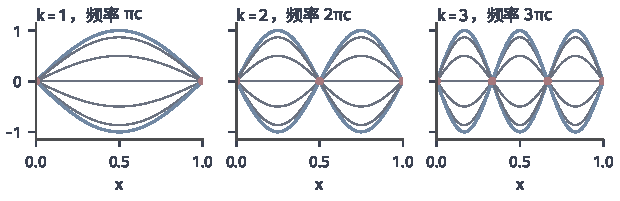
\includegraphics[width=105mm]{figures/03-optimization-evolution-and-signals/02-processes-and-trajectory-evolution/matplotlib/pde-standing-waves/figure.pdf}
  \caption{两端固定的弦的前三个驻波$\sin(k\pi x)\cos(k\pi ct)$。每幅图叠画了$k\pi ct=0,\pi/6,\ldots,\pi$七个时刻的形状，蓝色为最大位移；红点为节点$x=j/k$。模式不衰减，第$k$个模式的角频率为$k\pi c$。}
  \label{fig:pde-standing-waves}
\end{figure}

一般初值用$e_k=\sqrt2\sin(k\pi x)$展开：记$a_k=\langle u_0,e_k\rangle$、$b_k=\langle u_1,e_k\rangle$，
\begin{equation}
  u(t)=\sum_{k=1}^\infty\Bigl[a_k\cos(\omega_kt)+\frac{b_k}{\omega_k}\sin(\omega_kt)\Bigr]e_k .
  \label{eq:pde-wave-series}
\end{equation}
它在什么意义下是解，取决于初值的光滑程度。若$u_0\in H_0^1(0,1)$、$u_1\in L^2(0,1)$，则$\sum_kk^2\pi^2a_k^2=\|u_0'\|^2<\infty$（分部积分给出$\langle u_0',\sqrt2\cos(k\pi x)\rangle=k\pi a_k$，而$u_0'$的均值为零，再用余弦系的完备性与Parseval等式），$\sum b_k^2=\|u_1\|^2<\infty$，于是级数在$H_0^1$中、它的时间导数在$L^2$中关于$t$一致收敛；这是下一小节能量空间中的解。要得到经典解，需要系数衰减得更快，例如$\sum k^2|a_k|<\infty$与$\sum k|b_k|<\infty$可以保证逐项求两阶导数后一致收敛。

与热方程的定理~\ref{thm:pde-heat-series}对照，这里没有任何因子帮助级数收敛：$\cos(\omega_kt)$不衰减，初值有多粗糙，解在所有时刻就有多粗糙。拨弦时初始形状是三角形$u_0=\min(x,1-x)$，$a_k=2\sqrt2\sin(k\pi/2)/(k^2\pi^2)$只按$k^{-2}$衰减，$\sum k^2|a_k|$发散；三角形的尖角不会被磨平，而是分成两个折点，以速度$c$来回跑动、在两端反射，永远存在。形式上写出级数，不等于得到了经典解。

\subsection{能量估计与解的稳定性}
\label{sec:pde-wave-energy}

\paragraph{动能与势能}
弦的能量由两部分组成：动能$\tfrac12\int\rho u_t^2$与拉伸储存的弹性势能，后者在小斜率近似下为$\tfrac12\int Tu_x^2$。除以$\rho$，对$\Omega\subset\mathbb R^d$上的$u_{tt}=c^2\Delta u+f$定义
\begin{equation}
  E(t)=\frac12\int_\Omega\bigl(u_t^2+c^2|\nabla u|^2\bigr)\,\mathrm d\bm x .
  \label{eq:pde-wave-energy}
\end{equation}
设$u$足够光滑。对$t$求导，并对含$\nabla u\cdot\nabla u_t$的项用Green恒等式~\eqref{eq:pde-green-identity}，
\[
  E'(t)=\int_\Omega u_t\bigl(u_{tt}-c^2\Delta u\bigr)\,\mathrm d\bm x+c^2\int_{\partial\Omega}u_t\,\partial_{\bm n}u\,\mathrm dS
  =\int_\Omega fu_t\,\mathrm d\bm x+c^2\int_{\partial\Omega}u_t\,\partial_{\bm n}u\,\mathrm dS .
\]
边界项在两种常见条件下都消失：固定端$u=0$对所有$t$成立，所以边界上$u_t=0$；自由端$\partial_{\bm n}u=0$。于是无源时$E'(t)=0$，能量守恒：动能与势能来回转换，总量不变。

有源时，$E'=\langle f,u_t\rangle\leq\|f\|\,\|u_t\|\leq\|f\|\sqrt{2E}$。为了避免在$E=0$处除以零，对$\varepsilon>0$考察$\sqrt{E+\varepsilon}$：
\[
  \frac{\mathrm d}{\mathrm dt}\sqrt{E+\varepsilon}=\frac{E'}{2\sqrt{E+\varepsilon}}\leq\frac{\|f\|\sqrt{2E}}{2\sqrt{E+\varepsilon}}\leq\frac{\|f\|}{\sqrt2},
\]
积分后令$\varepsilon\to0$，得
\begin{equation}
  \sqrt{E(t)}\leq\sqrt{E(0)}+\frac1{\sqrt2}\int_0^t\|f(s)\|\,\mathrm ds .
  \label{eq:pde-wave-energy-source}
\end{equation}
源项注入的能量随时间累积，但不会被放大。

\paragraph{唯一性与连续依赖}
设$u_1,u_2$是同一问题的两个光滑解，差$w$满足无源方程、零初值与齐次边界条件。$w$的能量在$t=0$为零，又守恒，所以恒为零，于是$w_t=0$、$\nabla w=0$，$w$是常数；它的初值为零，所以$w\equiv0$。对数据不同的两个解，把式~\eqref{eq:pde-wave-energy-source}用于差，得到能量范数下的连续依赖：初位移的梯度、初速度和源项的小扰动，只引起位移梯度与速度的小变化。

这一估计也指出了波动方程自然的状态空间：位移属于$H_0^1$（或相应边界条件下的$H^1$），速度属于$L^2$，即$(u,u_t)\in H_0^1\times L^2$，能量正是这个乘积空间中的范数平方（差一个常数）。在这个空间中，可以仿照第~\ref{sec:pde-heat-semigroup}小节用Galerkin逼近定义并构造弱解，式~\eqref{eq:pde-wave-series}在$u_0\in H_0^1$、$u_1\in L^2$下给出的就是它。还要注意，把$t$换成$-t$，波动方程不变：由时刻$T$的位移和速度反推初值，与正向求解一样适定，这与反向热方程的严重不适定形成对照。

\paragraph{阻尼与耗散}
若弦在空气中振动，受到与速度成正比的阻力，方程变为$u_{tt}+\gamma u_t=c^2u_{xx}$，$\gamma>0$。同样的计算给出$E'=-\gamma\|u_t\|^2\leq0$，能量递减。逐个模式看，振幅满足$a''+\gamma a'+\omega_k^2a=0$；$\omega_k>\gamma/2$时振幅按$e^{-\gamma t/2}$衰减，能量大约按$e^{-\gamma t}$衰减，并带有动能与势能交替带来的起伏。

图~\ref{fig:pde-energy-compare}比较了三种情形的能量。无阻尼的波动能量是一条水平线；阻尼波动的能量沿$e^{-0.5t}$阶梯式下降，在速度为零的时刻（能量全部为势能）阻尼暂时不做功；热方程的能量单调衰减。

\begin{figure}[!htb]
  \centering
  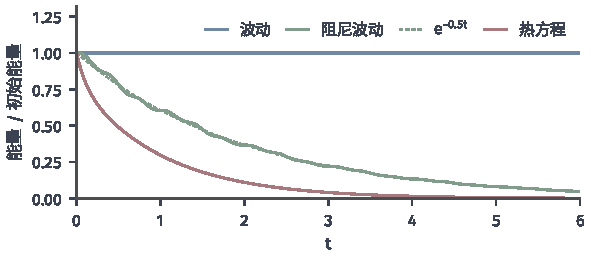
\includegraphics[width=100mm]{figures/03-optimization-evolution-and-signals/02-processes-and-trajectory-evolution/matplotlib/pde-energy-compare/figure.pdf}
  \caption{区间$(0,1)$上两端为零、初值$\sin(\pi x)+\tfrac12\sin(3\pi x)$的三种演化的能量，均相对初始能量归一化。波动方程$u_{tt}=u_{xx}$（初速度为零）的能量$\tfrac12\int(u_t^2+u_x^2)$守恒；阻尼波动$u_{tt}+0.5u_t=u_{xx}$的能量沿虚线$e^{-0.5t}$下降；热方程$u_t=0.05u_{xx}$的能量$\tfrac12\int u^2$单调衰减。曲线由精确的模式解计算。}
  \label{fig:pde-energy-compare}
\end{figure}

两种衰减的来源不同。热方程对时间是一阶的，能量等式~\eqref{eq:pde-heat-energy}中自动出现$-\|\nabla u\|^2$，耗散是方程结构本身带来的，不需要额外的项。无阻尼波动方程的能量等式中没有这样的项，能量严格守恒；衰减只能来自外加的阻尼。所以热方程的耗散结论、磨光效应与最大值原理都不能搬到波动方程上。最大值原理的失效有一个简单的例子：全直线上取$u_0=0$、$u_1\geq0$为一个非零鼓包，初始位移处处为零，由式~\eqref{eq:pde-dalembert}，$t>0$时在鼓包附近$u>0$，最大值并不在初始时刻取到。

% 第3章第6节：空间离散与数值解（有限差分与网格方程；Galerkin与有限元方法；时间推进与误差分配）。

\section{空间离散与数值解}
\label{sec:pde-discretization}

前面各节研究的是连续的场。计算机只能存储有限个数，所以要把场换成有限个未知量，把偏微分方程换成代数方程或常微分方程组。本节固定前面的方程和数据，研究两种空间离散：有限差分在网格点上逼近导数，有限元在有限维函数子空间上求弱形式。演化问题经空间离散后变成常微分方程组，再用第~\ref{chap:ordinary-differential-equations}章的时间推进方法求解。我们始终区分三个误差来源：空间离散的误差、时间推进的误差和代数方程没有解准的误差。

\subsection{有限差分与网格方程}
\label{sec:pde-finite-difference}

\paragraph{差商与网格未知量}
在$[0,1]$上取等距网格$x_j=jh$，$j=0,1,\ldots,N+1$，$h=1/(N+1)$。两端$x_0,x_{N+1}$是边界点，值由边界条件给出；内部的$N$个未知数$U_j$是对$u(x_j)$的近似。\term{有限差分方法}（finite difference method）把导数换成网格值的差商。对二阶导数，用中心差商
\[
  \delta_h^2u(x)=\frac{u(x+h)-2u(x)+u(x-h)}{h^2} .
\]
设$u\in C^4$，把$u(x\pm h)$在$x$处展开到四阶并带Lagrange余项，奇数阶项相互抵消，两个四阶余项由介值定理合并，得
\begin{equation}
  \delta_h^2u(x)=u''(x)+\frac{h^2}{12}u^{(4)}(\xi),\qquad\xi\in(x-h,x+h).
  \label{eq:pde-central-difference}
\end{equation}
差商以$h^2$的速度逼近二阶导数。这与式~\eqref{eq:pde-neighbor-average}是同一件事：二阶导数度量一点与两侧邻居平均值之差。

\paragraph{Poisson方程的网格方程}
对$-u''=f$、$u(0)=\alpha$、$u(1)=\beta$，在每个内部网格点上用差商代替二阶导数：
\[
  \frac{-U_{j-1}+2U_j-U_{j+1}}{h^2}=f(x_j),\qquad j=1,\ldots,N,\qquad U_0=\alpha,\ U_{N+1}=\beta .
\]
第一个和最后一个方程含有已知的边界值，把它们移到右端：第$1$行的右端变为$f(x_1)+\alpha/h^2$，第$N$行变为$f(x_N)+\beta/h^2$。记$\bm U=(U_1,\ldots,U_N)^{\top}$，得到线性方程组
\begin{equation}
  \bm A_h\bm U=\bm F,\qquad
  \bm A_h=\frac1{h^2}\begin{bmatrix}2&-1&&\\-1&2&\ddots&\\&\ddots&\ddots&-1\\&&-1&2\end{bmatrix}\in\mathbb R^{N\times N}.
  \label{eq:pde-fd-poisson}
\end{equation}
$\bm A_h$是对称三对角矩阵，每行至多三个非零元，共$3N-2$个；用三对角消元求解只需$O(N)$次运算。在单位正方形上用$N\times N$个内部网格点，五点格式$(4U_{i,j}-U_{i-1,j}-U_{i+1,j}-U_{i,j-1}-U_{i,j+1})/h^2=f_{i,j}$给出$N^2$个未知数，每行至多五个非零元。图~\ref{fig:pde-fd-stencil-sparsity}画出了一维模板和两种矩阵的非零元位置：矩阵很大，但几乎全是零。

\begin{figure*}[!htb]
  \centering
  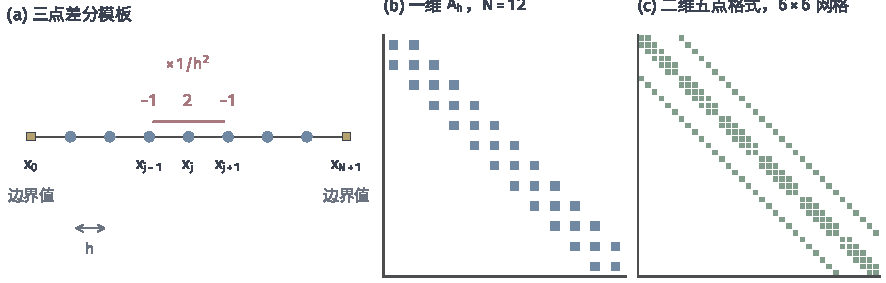
\includegraphics[width=150mm]{figures/03-optimization-evolution-and-signals/02-processes-and-trajectory-evolution/matplotlib/pde-fd-stencil-sparsity/figure.pdf}
  \caption{有限差分的网格与矩阵结构。(a)~一维网格：方块为已知的边界值，圆点为未知数；第$j$个方程用$x_{j-1},x_j,x_{j+1}$三点，权重为$(-1,2,-1)/h^2$。(b)~一维矩阵$\bm A_h$的非零元，$N=12$，三对角。(c)~单位正方形上$6\times6$内部网格的五点格式按行编号后的$36\times36$矩阵：主对角线两侧各有一条紧邻的副对角线（同一行的左右邻居）和一条相距$6$的副对角线（上下邻居）。}
  \label{fig:pde-fd-stencil-sparsity}
\end{figure*}

$\bm A_h$的特征向量可以直接写出。令$(\bm v_k)_j=\sin(k\pi x_j)$，$k=1,\ldots,N$。由$\sin(k\pi(x_j+h))+\sin(k\pi(x_j-h))=2\cos(k\pi h)\sin(k\pi x_j)$，且$\sin(k\pi x_0)=\sin(k\pi x_{N+1})=0$，
\[
  \bm A_h\bm v_k=\mu_k\bm v_k,\qquad\mu_k=\frac{2-2\cos(k\pi h)}{h^2}=\frac4{h^2}\sin^2\frac{k\pi h}{2} .
\]
离散的特征向量正是连续模式$\sin(k\pi x)$在网格上的取样。低频时$\mu_k\approx k^2\pi^2$，与连续的特征值一致；最高频$\mu_N\approx4/h^2$，远小于连续的$N^2\pi^2\approx\pi^2/h^2$，网格无法如实表示比两倍网格间距更短的波长。最大与最小特征值之比约为$4/(\pi^2h^2)$，网格越细，矩阵的条件数越大。

\paragraph{一致性：截断误差}
网格解$\bm U$离精确解有多远？第一步是问：把精确解代入网格方程，差多少。设$u\in C^4$是精确解，定义\term{截断误差}（truncation error）$\tau_j=(\bm A_h\bm u_h)_j-F_j$，其中$\bm u_h=(u(x_1),\ldots,u(x_N))^{\top}$。由式~\eqref{eq:pde-central-difference}与$-u''=f$，
\[
  \tau_j=-\delta_h^2u(x_j)+u''(x_j)=-\frac{h^2}{12}u^{(4)}(\xi_j),\qquad\|\bm\tau\|_\infty\leq\frac{h^2}{12}\|u^{(4)}\|_\infty .
\]
截断误差趋于零，称格式与方程一致。但这只说明精确解“几乎满足”网格方程，并没有说明网格方程的解接近精确解：若$\bm A_h^{-1}$的范数随$h\to0$无界增长，很小的$\bm\tau$也可能被放大成很大的误差。还需要一个与$h$无关的稳定估计。

\paragraph{稳定性：离散最大值原理}
连续问题有最大值原理，网格方程也有。

\begin{lemma}[离散最大值原理]
\label{lem:pde-discrete-max}
设$\bm V\in\mathbb R^N$，补充$V_0=V_{N+1}=0$。若$(\bm A_h\bm V)_j\geq0$对所有$j$成立，则$\bm V\geq\bm 0$（逐分量）。因此$\bm A_h$可逆，且$\bm A_h^{-1}$的元素全部非负。
\end{lemma}

\begin{proof}
设$m=\min_jV_j$在$j_*$处取到，反设$m<0$。由$(\bm A_h\bm V)_{j_*}\geq0$，$2m=2V_{j_*}\geq V_{j_*-1}+V_{j_*+1}\geq2m$，等号成立，两个邻居也等于$m$。逐步向左推，直到$j=1$：它的左邻居$V_0=0$也必须等于$m<0$，矛盾。所以$\bm V\geq\bm 0$。若$\bm A_h\bm V=\bm 0$，对$\bm V$与$-\bm V$分别使用结论得$\bm V=\bm 0$，$\bm A_h$可逆；对$\bm G\geq\bm 0$，$\bm V=\bm A_h^{-1}\bm G$满足条件，所以$\bm A_h^{-1}\bm G\geq\bm 0$。
\end{proof}

要得到定量的界，用一个比较函数。$w(x)=x(1-x)/2$是二次函数，式~\eqref{eq:pde-central-difference}中的余项为零，所以它的网格值$\bm w$精确满足$\bm A_h\bm w=\bm 1$，$\bm 1$为全一向量。对任意$\bm G$，向量$\|\bm G\|_\infty\bm w-\bm A_h^{-1}\bm G$经$\bm A_h$作用后为$\|\bm G\|_\infty\bm 1-\bm G\geq\bm 0$，由引理~\ref{lem:pde-discrete-max}它非负；同理$\|\bm G\|_\infty\bm w+\bm A_h^{-1}\bm G\geq\bm 0$。于是
\begin{equation}
  \|\bm A_h^{-1}\bm G\|_\infty\leq\|\bm G\|_\infty\max_jw_j\leq\frac18\|\bm G\|_\infty .
  \label{eq:pde-fd-stability}
\end{equation}
常数$1/8$与$h$无关。它是连续估计“$-u''=f$、两端为零时$\|u\|_\infty\leq\|f\|_\infty/8$”在网格上的复制品。

\paragraph{收敛：一致性加稳定性}
把两步合起来。误差$\bm e=\bm u_h-\bm U$满足$\bm A_h\bm e=\bm A_h\bm u_h-\bm F=\bm\tau$，由式~\eqref{eq:pde-fd-stability}得到下面的结论。

\begin{theorem}[一维Poisson差分格式的收敛]
\label{thm:pde-fd-convergence}
设$f$连续，$-u''=f$配Dirichlet边界条件的解$u\in C^4([0,1])$，$\bm U$为网格方程~\eqref{eq:pde-fd-poisson}的解。则
\[
  \max_{1\leq j\leq N}|u(x_j)-U_j|\leq\frac{h^2}{96}\|u^{(4)}\|_\infty .
\]
\end{theorem}

以$u=\sin(\pi x)$、$f=\pi^2\sin(\pi x)$为例，界为$\pi^4h^2/96\approx1.01h^2$。$N=4$、$h=0.2$时实际最大误差约$0.032$，界为$0.041$。图~\ref{fig:pde-convergence}中蓝色折线是$N$从$4$到$256$的实际误差，在对数坐标下斜率为$2.00$，与定理给出的阶一致。“一致性加稳定性推出收敛”是数值分析的一般原理；对线性问题，Lax等价定理把它表述为：一致的格式收敛当且仅当它稳定。这里的稳定性属于具体的格式与具体的范数，换一个格式或换一个范数需要重新证明。

\paragraph{热方程的半离散}
对热方程$u_t=\kappa u_{xx}+f$，只在空间上离散，时间保持连续：
\begin{equation}
  \bm U'(t)=-\kappa\bm A_h\bm U(t)+\bm F(t),\qquad\bm U(0)=\bigl(u_0(x_1),\ldots,u_0(x_N)\bigr)^{\top}.
  \label{eq:pde-semidiscrete-heat}
\end{equation}
这是一个$N$维线性常微分方程组，这种先离散空间、再处理时间的做法称为\term{方法线}（method of lines）。它的第$k$个特征分量以速率$\kappa\mu_k$衰减：低频模式的衰减率接近连续的$\kappa k^2\pi^2$，高频模式的衰减率被低估，但它们本来就在极短时间内衰减殆尽。空间误差就是半离散系统与连续解之差，下一小节在具体例子中把它与时间误差分开。

\subsection{Galerkin与有限元方法}
\label{sec:pde-fem}

有限差分直接逼近方程中的导数，要求解足够光滑才能用Taylor展开估计误差。另一条路线从弱形式出发：不逼近方程，而是在一个有限维函数空间中求弱形式的解。这条路线天然适合粗糙数据和不规则区域，误差分析也直接建立在第~\ref{sec:pde-poisson}节的能量框架上。

\paragraph{在有限维子空间上求弱形式}
设$V_h\subset H_0^1(\Omega)$是有限维子空间。\term{Galerkin方法}（Galerkin method）求$u_h\in V_h$，使
\begin{equation}
  a(u_h,v_h)=\ell(v_h)\qquad\text{对所有}v_h\in V_h .
  \label{eq:pde-galerkin}
\end{equation}
它只是把弱形式~\eqref{eq:pde-weak-dirichlet}中的解空间和检验空间同时换成$V_h$。取$V_h$的基$\varphi_1,\ldots,\varphi_n$，写$u_h=\sum_jc_j\varphi_j$，并依次取$v_h=\varphi_i$，得到线性方程组
\[
  \bm K\bm c=\bm F,\qquad\bm K_{i,j}=a(\varphi_j,\varphi_i),\qquad\bm F_i=\ell(\varphi_i).
\]
对Poisson方程，$\bm c^{\top}\bm K\bm c=a(v_h,v_h)=\|\nabla v_h\|^2>0$对非零的$v_h=\sum c_j\varphi_j$成立，$\bm K$对称正定，方程组有唯一解。由第~\ref{sec:pde-weak-form}小节的能量对应，$u_h$也是能量$J$在$V_h$上的最小点，这时称为Ritz方法；在有限维中求二次函数的最小点是第~\ref{chap:optimization}章已经处理过的问题。新的问题是：$u_h$与真正的解$u$相差多少。

\paragraph{帽函数与刚度矩阵}
一维时取与上一小节相同的网格，令
\[
  \varphi_j(x)=\max\Bigl(0,\,1-\frac{|x-x_j|}{h}\Bigr),\qquad j=1,\ldots,N .
\]
$\varphi_j$是在$x_j$处取$1$、在其余网格点取$0$、在每个小区间上线性的\term{帽函数}（hat function）。它们张成的$V_h$恰好是两端为零的连续分片线性函数全体，并且$v_h=\sum_jv_h(x_j)\varphi_j$：系数就是网格点上的值。用分片多项式基构造Galerkin空间的方法称为\term{有限元方法}（finite element method）。

两个帽函数只有在相邻时支撑才重叠，所以矩阵是三对角的。$\varphi_j'$在$(x_{j-1},x_j)$上为$1/h$、在$(x_j,x_{j+1})$上为$-1/h$，直接积分得$\bm K_{j,j}=2/h$、$\bm K_{j,j\pm1}=-1/h$，即\term{刚度矩阵}（stiffness matrix）$\bm K=h\bm A_h$。若把载荷$\bm F_i=\int f\varphi_i$近似为$f(x_i)\int\varphi_i=hf(x_i)$，方程$\bm K\bm c=\bm F$就变成$\bm A_h\bm c=(f(x_i))_i$，与有限差分格式~\eqref{eq:pde-fd-poisson}完全相同。两种方法出发点不同，在这个最简单的情形中给出同一组方程；区别在于有限元的误差分析来自弱形式，可以直接推广到粗糙数据、非均匀网格和高维的三角形网格。图~\ref{fig:pde-fem-hats}(a)画出了$h=1/6$时的五个帽函数。

\begin{figure}[!htb]
  \centering
  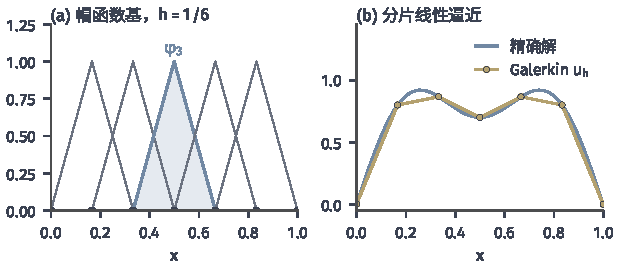
\includegraphics[width=105mm]{figures/03-optimization-evolution-and-signals/02-processes-and-trajectory-evolution/matplotlib/pde-fem-hats/figure.pdf}
  \caption{一维有限元。(a)~$h=1/6$时的帽函数基，蓝色阴影为$\varphi_3$，每个帽函数只与相邻两个重叠。(b)~$-u''=f$、两端为零的精确解$u=\sin(\pi x)+0.3\sin(3\pi x)$与Galerkin解$u_h$，载荷积分精确计算；$u_h$在网格点上与$u$相同（数值误差约$7\times10^{-10}$），在网格点之间线性插值。}
  \label{fig:pde-fem-hats}
\end{figure}

\paragraph{组装、边界条件与积分近似}
实际计算中，$\bm K$按单元逐块组装：在每个小区间上，两个局部基函数给出$2\times2$的单元矩阵$\tfrac1h\bigl[\begin{smallmatrix}1&-1\\-1&1\end{smallmatrix}\bigr]$，把它加到全局矩阵的对应位置即可。高维的三角形单元同样处理，只是单元矩阵由三角形的几何决定。

计算流程中的每一个环节对应一种近似，分别改变不同的对象。选$V_h$决定了用什么函数逼近解，这是空间离散。非零Dirichlet数据把边界节点的值固定，并把它们的贡献移到右端；Neumann数据则保留边界节点为未知数，把边界积分$\int g v_h$加入载荷，自然边界条件在这里不需要额外处理。用数值积分计算$\bm F_i$或$\bm K_{i,j}$，相当于把$\ell$或$a$换成近似的$\ell_h$或$a_h$，解的是一个略有不同的问题，它带来的误差可以用$\sup_{v_h}|\ell(v_h)-\ell_h(v_h)|/\|\nabla v_h\|$控制（第一Strang引理）。最后，用迭代法解$\bm K\bm c=\bm F$时在残差足够小处停止，系数误差是$\bm K^{-1}$作用在残差上的结果。

\paragraph{Galerkin正交性与Céa引理}
从$a(u,v)=\ell(v)$（对所有$v\in V$）中取$v=v_h\in V_h$，减去式~\eqref{eq:pde-galerkin}，得到
\begin{equation}
  a(u-u_h,v_h)=0\qquad\text{对所有}v_h\in V_h ,
  \label{eq:pde-galerkin-orthogonality}
\end{equation}
称为\term{Galerkin正交性}（Galerkin orthogonality）。对称情形中$a$是内积，它说误差$u-u_h$与整个$V_h$在能量内积下正交，所以$u_h$是$u$在$V_h$上的能量正交投影，在能量范数下离$u$最近。一般情形有下面的结论。

\begin{theorem}[Céa引理]
\label{thm:pde-cea}
设$V$为Hilbert空间，$a$满足有界性与强制性~\eqref{eq:pde-bounded-coercive}，$V_h\subset V$为闭子空间，$u$与$u_h$分别为$V$与$V_h$上的Galerkin解。则
\[
  \|u-u_h\|_V\leq\frac M\alpha\inf_{v_h\in V_h}\|u-v_h\|_V .
\]
\end{theorem}

\begin{proof}
对任意$v_h\in V_h$，$u_h-v_h\in V_h$，由式~\eqref{eq:pde-galerkin-orthogonality}，$a(u-u_h,u_h-v_h)=0$。于是
\[
  \begin{aligned}
    \alpha\|u-u_h\|_V^2&\leq a(u-u_h,u-u_h)=a(u-u_h,u-v_h)\\
    &\leq M\|u-u_h\|_V\|u-v_h\|_V ,
  \end{aligned}
\]
约去$\|u-u_h\|_V$，再对$v_h$取下确界。
\end{proof}

Céa引理把“Galerkin解有多准”化成了“$V_h$中最好的逼近有多准”，后者只是一个逼近论问题，与方程无关。对Poisson方程取$\|v\|_V=\|\nabla v\|$，$M=\alpha=1$，Galerkin解就是最优逼近。一维时还有一个更强的事实：$u_h$在网格点上与$u$完全相同。由例~\ref{ex:pde-point-source}，Green函数$G(\cdot,x_j)$满足$a(G(\cdot,x_j),v)=v(x_j)$；它在$x_j$处有折点、在其余处线性、两端为零，所以属于$V_h$。取$v=u-u_h$并用对称性与Galerkin正交性，$u(x_j)-u_h(x_j)=a(u-u_h,G(\cdot,x_j))=0$。图~\ref{fig:pde-fem-hats}(b)中的Galerkin解正是$u$的分片线性插值。这一性质依赖一维Green函数是分片线性的，高维中不成立。

\paragraph{逼近性质给出误差阶}
剩下的问题是分片线性函数能多好地逼近$u$。记$I_hu$为$u$在网格点上的分片线性插值。

\begin{lemma}[分片线性插值的误差]
\label{lem:pde-interpolation}
设$u\in H^2(0,1)\cap H_0^1(0,1)$，则$\|(u-I_hu)'\|\leq(h/\pi)\|u''\|$。
\end{lemma}

\begin{proof}
在一个单元$K=[x_j,x_{j+1}]$上，$e=u-I_hu$在两端为零，所以$\int_Ke'=0$，$e'$在$K$上均值为零。$I_hu$在$K$上线性，$e''=u''$。对$e'\in H^1(K)$用长度为$h$的区间上零均值的Poincaré不等式，第~\ref{sec:pde-boundary-solution-meaning}小节回顾过其最优常数为$h/\pi$，得$\|e'\|_{L^2(K)}\leq(h/\pi)\|u''\|_{L^2(K)}$。对所有单元平方求和即得。
\end{proof}

由Céa引理，$\|(u-u_h)'\|\leq\|(u-I_hu)'\|\leq(h/\pi)\|u''\|=(h/\pi)\|f\|$：能量范数下误差为$O(h)$。$L^2$范数下误差更小，可以用对偶论证得到。记$e=u-u_h$，令$z\in H_0^1$为$-z''=e$的弱解；由定理~\ref{thm:pde-regularity-1d}，$z\in H^2$且$\|z''\|=\|e\|$。在$z$的弱形式中取检验函数$e$，再用Galerkin正交性减去$I_hz\in V_h$，
\[
  \|e\|^2=a(z,e)=a(e,z-I_hz)\leq\|e'\|\,\|(z-I_hz)'\|\leq\|e'\|\cdot\frac h\pi\|e\| ,
\]
所以$\|e\|\leq(h/\pi)\|e'\|\leq(h^2/\pi^2)\|f\|$，$L^2$误差为$O(h^2)$。图~\ref{fig:pde-convergence}中绿色与黄色折线是$u=\sin(\pi x)$时的两种误差，拟合斜率分别为$1.00$与$2.00$。$h=0.2$时能量误差约$0.40$，而界$(h/\pi)\|u''\|=0.2\pi/\sqrt2\approx0.44$，已相当接近实际值。

\begin{figure}[!htb]
  \centering
  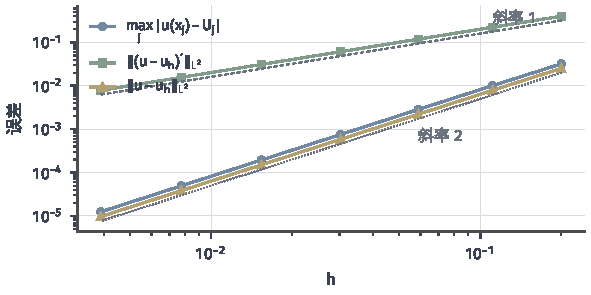
\includegraphics[width=100mm]{figures/03-optimization-evolution-and-signals/02-processes-and-trajectory-evolution/matplotlib/pde-convergence/figure.pdf}
  \caption{$-u''=\pi^2\sin(\pi x)$、两端为零时的误差随网格尺寸$h=1/(N+1)$的变化，$N=4,8,\ldots,256$，双对数坐标。蓝色：有限差分网格值的最大误差；绿色：有限元解导数的$L^2$误差；黄色：有限元解的$L^2$误差（载荷精确积分，单元上用$8$点Gauss求积计算误差）。灰色虚线与点线为斜率$1$与$2$的参考线。}
  \label{fig:pde-convergence}
\end{figure}

这两个阶都依赖$u\in H^2$。在高维的三角形网格上，类似的插值估计与Céa引理同样给出能量误差$O(h)$，但前提仍是解属于$H^2$；第~\ref{sec:pde-lax-milgram}小节L形区域凹角处的解不在$H^2$中，均匀网格上的收敛阶会相应降低，需要在凹角附近加密网格。误差阶来自“方程的稳定性（Céa引理）乘以解的可逼近性（插值估计）”，二者缺一不可。

\subsection{时间推进与误差分配}
\label{sec:pde-time-stepping}

\paragraph{半离散系统与刚性}
空间离散后的热方程是常微分方程组~\eqref{eq:pde-semidiscrete-heat}；有限元给出$\bm M\bm c'+\kappa\bm K\bm c=\bm F$，其中$\bm M_{i,j}=\langle\varphi_j,\varphi_i\rangle$是质量矩阵。矩阵$-\kappa\bm A_h$的特征值$-\kappa\mu_k$分布在约$-\kappa\pi^2$到$-4\kappa/h^2$之间，最快与最慢衰减率之比约为$4/(\pi^2h^2)$：$h=0.01$时约为$4000$。按第~\ref{chap:ordinary-differential-equations}章的说法，这是一个刚性问题：真正关心的是缓慢衰减的低频模式，最快的模式却限制了显式方法的步长。

\paragraph{显式Euler与扩散步长条件}
用步长$\Delta t$做显式Euler，$\bm U^{(n+1)}=\bm U^{(n)}-\Delta t\,\kappa\bm A_h\bm U^{(n)}$，逐点写出来是
\begin{equation}
  U_j^{(n+1)}=U_j^{(n)}+r\bigl(U_{j-1}^{(n)}-2U_j^{(n)}+U_{j+1}^{(n)}\bigr),\qquad r=\frac{\kappa\Delta t}{h^2} .
  \label{eq:pde-explicit-heat}
\end{equation}
第$k$个特征分量每步乘以放大因子$g_k=1-\Delta t\,\kappa\mu_k=1-4r\sin^2(k\pi h/2)$。所有分量不增长要求$|g_k|\leq1$，即$4r\sin^2(k\pi h/2)\leq2$对所有$k\leq N$成立；$r\leq1/2$时它对任何网格成立，而$h\to0$时$\sin^2(N\pi h/2)\to1$，所以$r$略大于$1/2$就会让最高频分量增长。这就是扩散问题显式格式的步长条件$\Delta t\leq h^2/(2\kappa)$。

$r\leq1/2$还有一个直接的读法：式~\eqref{eq:pde-explicit-heat}可写为$U_j^{(n+1)}=rU_{j-1}^{(n)}+(1-2r)U_j^{(n)}+rU_{j+1}^{(n)}$，三个系数非负且和为$1$，新值是旧值的凸组合，所以网格上的最大值不增、最小值不减，这是热方程最大值原理的离散版本。$r>1/2$时中间系数为负，凸组合的解释失效。图~\ref{fig:pde-explicit-stability}比较了$r=0.48$与$r=0.52$：初值是$\sin(\pi x)$加上振幅$0.01$的锯齿扰动，前者的锯齿迅速消失，后者的锯齿每步反号并放大，$60$步后最大值已约为$1.09$，而真解此时约为$0.46$。

\begin{figure*}[!htb]
  \centering
  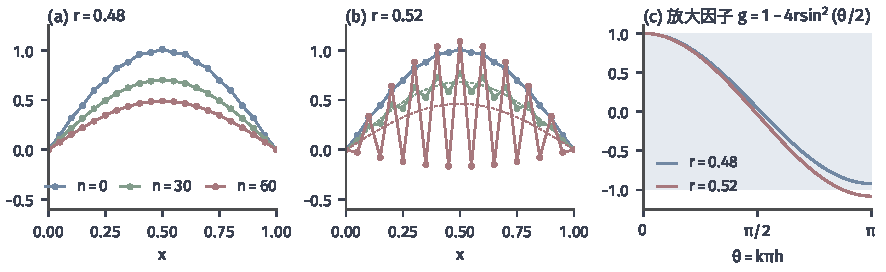
\includegraphics[width=150mm]{figures/03-optimization-evolution-and-signals/02-processes-and-trajectory-evolution/matplotlib/pde-explicit-stability/figure.pdf}
  \caption{热方程显式格式~\eqref{eq:pde-explicit-heat}的稳定与失稳，$h=1/20$，初值$\sin(\pi x_j)+0.01(-1)^j$。(a)~$r=0.48$：第$0,30,60$步的网格解（带点折线）紧贴同时刻的真解$e^{-\pi^2t}\sin(\pi x)$（同色虚线）。(b)~$r=0.52$：高频锯齿逐步放大，第$60$步最大值约$1.09$。(c)~放大因子$g=1-4r\sin^2(\theta/2)$随离散频率$\theta=k\pi h$的变化，浅蓝带为$|g|\leq1$；$r=0.52$的曲线在高频端越出$-1$。}
  \label{fig:pde-explicit-stability}
\end{figure*}

这个条件的代价随网格加细迅速增长：$h$减半，步长须缩为四分之一，总步数增为四倍，每步的工作量又增为两倍。限制步长的是稳定性，不是精度：$r\leq1/2$时，最高频模式无论如何都会被正确地衰减掉，却仍然决定了整个计算的步长。

\paragraph{隐式格式：后向Euler与梯形法}
后向Euler在新时刻计算导数：$(\bm I+\Delta t\,\kappa\bm A_h)\bm U^{(n+1)}=\bm U^{(n)}$。放大因子$g_k=1/(1+\Delta t\,\kappa\mu_k)\in(0,1)$对任何$\Delta t$都成立，格式无条件稳定，且对高频模式强烈衰减；代价是每步解一个三对角方程组，仍只需$O(N)$次运算。梯形法（在偏微分方程中常称Crank--Nicolson格式）取两端的平均，$g_k=(1-z_k/2)/(1+z_k/2)$，$z_k=\Delta t\,\kappa\mu_k$。它对所有$z_k\geq0$满足$|g_k|<1$，也无条件稳定，时间精度为二阶，而后向Euler只有一阶；但$z_k\to\infty$时$g_k\to-1$，步长较大时高频模式几乎不衰减、每步反号。所以“无条件稳定”不等于“强烈阻尼”，初值粗糙时梯形法的解可能出现长时间残留的小振荡。

\paragraph{波动方程与CFL条件}
对$u_{tt}=c^2u_{xx}$，时间与空间都用中心差商，得到跳蛙格式
\[
  U_j^{(n+1)}-2U_j^{(n)}+U_j^{(n-1)}=\nu^2\bigl(U_{j-1}^{(n)}-2U_j^{(n)}+U_{j+1}^{(n)}\bigr),\qquad\nu=\frac{c\Delta t}{h} .
\]
代入$U_j^{(n)}=g^n\sin(k\pi x_j)$，记$s=\sin^2(k\pi h/2)$，得$g^2-2(1-2\nu^2s)g+1=0$。两根之积为$1$。若$|1-2\nu^2s|\leq1$，两根是模为$1$的共轭复数（或重根），模式既不增长也不衰减，正如连续的波动方程保持能量；若$1-2\nu^2s<-1$，即$\nu^2s>1$，两根为实数且其中一个的绝对值大于$1$，模式指数增长。由于$s<1$，$\nu\leq1$保证所有模式稳定；而$h\to0$时最高频的$s\to1$，$\nu$略大于$1$就会失稳。$\nu\leq1$称为\term{CFL条件}（Courant--Friedrichs--Lewy condition）。

它有一个与第~\ref{sec:pde-wave-solution}小节相呼应的几何解释。跳蛙格式第$n$步在$x_j$处的值只依赖初始网格值在$[x_j-nh,x_j+nh]$中的部分，这是数值的依赖区域；真解依赖的是$[x_j-cn\Delta t,x_j+cn\Delta t]$。若$c\Delta t>h$，真解的依赖区域超出了数值的依赖区域，改变超出部分的初始数据会改变真解而不改变数值解，格式不可能收敛。所以数值依赖区域必须包含真解的依赖区域，这是收敛的必要条件。对输运方程$u_t+bu_x=0$（$b>0$），\term{迎风格式}（upwind scheme）$U_j^{(n+1)}=U_j^{(n)}-\nu(U_j^{(n)}-U_{j-1}^{(n)})$、$\nu=b\Delta t/h$，在$0\leq\nu\leq1$时是$U_{j-1}^{(n)}$与$U_j^{(n)}$的凸组合，因而稳定；改用下游的$U_{j+1}^{(n)}$则对任何$\nu>0$都不稳定，因为信息来自上游，这与第~\ref{sec:pde-characteristics}小节只在流入边界给数据是同一个道理。

\paragraph{误差分配}
在终止时刻，总误差可以拆成几部分：连续解与半离散解之差是空间误差，对二阶差分为$O(h^2)$；半离散解与时间推进结果之差是时间误差，后向Euler为$O(\Delta t)$、梯形法为$O(\Delta t^2)$；每步隐式方程只解到某个残差时，还有代数误差；此外是舍入误差。总误差不超过各部分之和，计算量则由网格点数与步数共同决定。

图~\ref{fig:pde-error-plateau}用一个可以精确计算的例子显示这种分配。取$u_t=u_{xx}$、两端为零、$u_0=\sin(\pi x)$，在$t=0.1$比较网格解与真解$e^{-\pi^2t}\sin(\pi x)$。由于$\sin(\pi x_j)$恰是$\bm A_h$的特征向量，所有误差都可以写成显式的标量公式。固定$h$，减小$\Delta t$时后向Euler的误差先按$\Delta t$线性下降，然后停在一个平台上：平台高度是空间误差，$h=1/10,1/20,1/40$时分别约为$3.0\times10^{-3}$、$7.6\times10^{-4}$、$1.9\times10^{-4}$，每次减半$h$降为约四分之一。到达平台后再减小$\Delta t$只是浪费计算。梯形法用大得多的步长就到达平台；它的曲线在某处出现向下的尖谷，是因为时间误差与空间误差符号相反、在那里恰好抵消，并不说明那个步长有特殊的精度。

\begin{figure}[!htb]
  \centering
  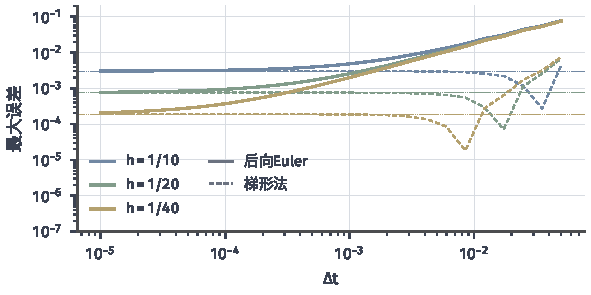
\includegraphics[width=100mm]{figures/03-optimization-evolution-and-signals/02-processes-and-trajectory-evolution/matplotlib/pde-error-plateau/figure.pdf}
  \caption{热方程$u_t=u_{xx}$、$u_0=\sin(\pi x)$在$t=0.1$时网格解的最大误差随时间步长的变化。三种颜色对应$h=1/10,1/20,1/40$；实线为后向Euler，虚线为梯形法；水平点线为同一$h$下半离散系统的空间误差。误差在$\Delta t$足够小后停在空间误差的平台上。}
  \label{fig:pde-error-plateau}
\end{figure}

两种误差平衡时计算量最省。后向Euler要让$O(\Delta t)$与$O(h^2)$相当，需取$\Delta t\sim h^2$，步数与显式格式的稳定限制同阶，只是现在是精度要求；梯形法只需$\Delta t\sim h$。网格加密一倍，前者的总工作量约增为八倍，后者约增为四倍。

最后是残差与误差的关系。迭代求解$\bm B\bm x=\bm b$时，常在残差$\bm r=\bm b-\bm B\tilde{\bm x}$足够小时停止；误差$\bm x-\tilde{\bm x}=\bm B^{-1}\bm r$，所以残差小能否推出误差小，取决于$\|\bm B^{-1}\|$。对后向Euler的矩阵$\bm I+\Delta t\,\kappa\bm A_h$，特征值不小于$1$，$\|\bm B^{-1}\|_2\leq1$，误差不超过残差；对Poisson矩阵，式~\eqref{eq:pde-fd-stability}给出最大范数下误差不超过残差的$1/8$。但若只控制相对残差，相对误差可能放大到条件数倍，而$\bm A_h$的条件数约为$4/(\pi^2h^2)$：$h=10^{-3}$时，$10^{-6}$的相对残差只保证约$0.4$的相对误差。残差小要经过相应的稳定估计，才能解释为解的误差小。

% 第3章第7节：本章小结。

\section{本章小结}
\label{sec:pde-summary}

本章开头问了四个问题：哪些数据确定一个场，粗糙数据下“满足方程”是什么意思，三种演化机制各自做了什么，网格上的近似何时可靠。下面按这四个问题收束。

\paragraph{四个代表方程的对照}
表~\ref{tab:pde-four-equations}把四个方程放在一起。Poisson方程描述平衡，在整个边界上给数据，解属于$H^1$类空间，Lax--Milgram定理与能量估计给出存在、唯一与连续依赖；边界条件一变，解空间、相容条件和唯一性随之改变。热方程描述耗散：它需要初值和整个边界上的数据，正弦模式按$e^{-k^2\pi^2t}$衰减，高频先消失，解在正时刻立即变光滑，能量单调减少，最大值原理成立，反向求解不适定。输运方程描述搬运：沿特征线它化为常微分方程，只在流入边界给数据，间断被原样搬走；守恒形式还要计入流动的压缩，非线性时特征线可能相交并产生激波。波动方程描述传播：需要位移与速度两个初值，信号以有限速度$c$传播，能量守恒，粗糙的初值永远不会被磨平，反向求解与正向一样适定。

\begin{table*}[!htb]
  \centering
  \begin{tabularx}{\linewidth}{@{}l>{\RaggedRight\arraybackslash}X>{\RaggedRight\arraybackslash}X>{\RaggedRight\arraybackslash}X>{\RaggedRight\arraybackslash}X@{}}
    \toprule
    方程 & 所需数据 & 解的自然空间 & 关键估计或性质 & 信息传递 \\
    \midrule
    Poisson $-\Delta u=f$ & 源项，整个边界 & $H_0^1$或$H^1$ & 强制性与能量估计 & 平衡，无时间 \\
    热方程 $u_t=\kappa\Delta u+f$ & 初值，整个边界 & 时间上取值于$H_0^1$ & 能量耗散，最大值原理 & 无穷速度，磨光 \\
    输运 $u_t+\bm b\cdot\nabla u=0$ & 初值，流入边界 & 沿特征线的$C^1$或弱解 & 沿特征线保值 & 沿特征线，不磨光 \\
    波动 $u_{tt}=c^2\Delta u$ & 初位移与初速度，整个边界 & $(u,u_t)\in H_0^1\times L^2$ & 能量守恒 & 有限速度$c$，不磨光 \\
    \bottomrule
  \end{tabularx}
  \caption{本章四个代表方程的对照（线性情形，有界区域或全直线）。}
  \label{tab:pde-four-equations}
\end{table*}

\paragraph{连续场、弱方程与有限维近似}
贯穿全章的工具是弱形式：用测试函数检验方程，把导数转移到测试函数上。它让源项可以只是可积函数甚至一维中的点源，让边界条件分成写进解空间的本质条件和藏在边界积分里的自然条件，也让能量估计成为证明唯一性与连续依赖的统一方法。同一个弱形式又直接给出数值方法：把解空间和检验空间同时换成有限维子空间，就是Galerkin与有限元方法；Galerkin正交性和Céa引理把数值误差归结为子空间的逼近能力。有限差分从另一端出发，用截断误差衡量一致性，用离散最大值原理证明稳定性，二者合起来给出收敛。演化问题经空间离散后成为刚性的常微分方程组，显式格式受$\Delta t\leq h^2/(2\kappa)$或CFL条件$c\Delta t\leq h$的限制，隐式格式解除了稳定性限制，但需要按精度平衡空间与时间误差。

\paragraph{几种不同的命题}
本章反复区分了几类结论，它们不能互相代替。写出弱形式或Euler--Lagrange方程，只说明“若有解，它满足什么”，不等于证明了解存在；存在与唯一需要Lax--Milgram定理这样的论证。形式级数只说明模式怎样组合，在什么空间中收敛、能否逐项求导，取决于初值的光滑程度。能量等式说明某个量守恒或衰减，它给出唯一性与连续依赖，但不直接给出逐点的光滑性。截断误差小只说明精确解几乎满足网格方程；离散解收敛到连续解，还需要与网格无关的稳定估计。残差小也只有经过相应的稳定估计，才能解释为误差小。

\paragraph{与后续章节的联系}
本章始终处理确定性的场。第~\ref{chap:continuous-time-stochastic-processes}章将看到，随机状态的概率密度怎样随时间演化：只有漂移时，密度满足本章的连续性方程；加入Brown运动的随机扰动后，密度满足带扩散项的方程，热方程就是其中最简单的情形。届时需要的确定性方程、弱解与半群语言都已在本章建立，随机过程一侧只需补充生成元与转移概率之间的联系。

